% ----------------------------------------------------------------------
%
%                            TFMTesis.tex
%
%----------------------------------------------------------------------
%
% Este fichero contiene el "documento maestro" del documento. Lo único
% que hace es configurar el entorno LaTeX e incluir los ficheros .tex
% que contienen cada sección.
%
%----------------------------------------------------------------------
%
% Los ficheros necesarios para este documento son:
%
%       TeXiS/* : ficheros de la plantilla TeXiS.
%       Cascaras/* : ficheros con las partes del documento que no
%          son capítulos ni apéndices (portada, agradecimientos, etc.)
%       Capitulos/*.tex : capítulos de la tesis
%       Apendices/*.tex: apéndices de la tesis
%       constantes.tex: constantes LaTeX
%       config.tex : configuración de la "compilación" del documento
%       guionado.tex : palabras con guiones
%
% Para la bibliografía, además, se necesitan:
%
%       *.bib : ficheros con la información de las referencias
%
% ---------------------------------------------------------------------

\documentclass[11pt,a4paper,twoside]{book}

%
% Definimos  el   comando  \compilaCapitulo,  que   luego  se  utiliza
% (opcionalmente) en config.tex. Quedaría  mejor si también se definiera
% en  ese fichero,  pero por  el modo  en el  que funciona  eso  no es
% posible. Puedes consultar la documentación de ese fichero para tener
% más  información. Definimos también  \compilaApendice, que  tiene el
% mismo  cometido, pero  que se  utiliza para  compilar  únicamente un
% apéndice.
%
%
% Si  queremos   compilar  solo   una  parte  del   documento  podemos
% especificar mediante  \includeonly{...} qué ficheros  son los únicos
% que queremos  que se incluyan.  Esto  es útil por  ejemplo para sólo
% compilar un capítulo.
%
% El problema es que todos aquellos  ficheros que NO estén en la lista
% NO   se  incluirán...  y   eso  también   afecta  a   ficheros  de
% la plantilla...
%
% Total,  que definimos  una constante  con los  ficheros  que siempre
% vamos a querer compilar  (aquellos relacionados con configuración) y
% luego definimos \compilaCapitulo.
\newcommand{\ficherosBasicosTeXiS}{%
TeXiS/TeXiS_pream,TeXiS/TeXiS_cab,TeXiS/TeXiS_bib,TeXiS/TeXiS_cover%
}
\newcommand{\ficherosBasicosTexto}{%
constantes,guionado,Cascaras/bibliografia,config%
}
\newcommand{\compilaCapitulo}[1]{%
\includeonly{\ficherosBasicosTeXiS,\ficherosBasicosTexto,Capitulos/#1}%
}

\newcommand{\compilaApendice}[1]{%
\includeonly{\ficherosBasicosTeXiS,\ficherosBasicosTexto,Apendices/#1}%
}

%- - - - - - - - - - - - - - - - - - - - - - - - - - - - - - - - - - -
%            Preámbulo del documento. Configuraciones varias
%- - - - - - - - - - - - - - - - - - - - - - - - - - - - - - - - - - -

% Define  el  tipo  de  compilación que  estamos  haciendo.   Contiene
% definiciones  de  constantes que  cambian  el  comportamiento de  la
% compilación. Debe incluirse antes del paquete TeXiS/TeXiS.sty
%---------------------------------------------------------------------
%
%                          config.tex
%
%---------------------------------------------------------------------
%
% Contiene la  definición de constantes  que determinan el modo  en el
% que se compilará el documento.
%
%---------------------------------------------------------------------
%
% En concreto, podemos  indicar si queremos "modo release",  en el que
% no  aparecerán  los  comentarios  (creados  mediante  \com{Texto}  o
% \comp{Texto}) ni los "por  hacer" (creados mediante \todo{Texto}), y
% sí aparecerán los índices. El modo "debug" (o mejor dicho en modo no
% "release" muestra los índices  (construirlos lleva tiempo y son poco
% útiles  salvo  para   la  versión  final),  pero  sí   el  resto  de
% anotaciones.
%
% Si se compila con LaTeX (no  con pdflatex) en modo Debug, también se
% muestran en una esquina de cada página las entradas (en el índice de
% palabras) que referencian  a dicha página (consulta TeXiS_pream.tex,
% en la parte referente a show).
%
% El soporte para  el índice de palabras en  TeXiS es embrionario, por
% lo  que no  asumas que  esto funcionará  correctamente.  Consulta la
% documentación al respecto en TeXiS_pream.tex.
%
%
% También  aquí configuramos  si queremos  o  no que  se incluyan  los
% acrónimos  en el  documento final  en la  versión release.  Para eso
% define (o no) la constante \acronimosEnRelease.
%
% Utilizando \compilaCapitulo{nombre}  podemos también especificar qué
% capítulo(s) queremos que se compilen. Si no se pone nada, se compila
% el documento  completo.  Si se pone, por  ejemplo, 01Introduccion se
% compilará únicamente el fichero Capitulos/01Introduccion.tex
%
% Para compilar varios  capítulos, se separan sus nombres  con comas y
% no se ponen espacios de separación.
%
% En realidad  la macro \compilaCapitulo  está definida en  el fichero
% principal tesis.tex.
%
%---------------------------------------------------------------------


% Comentar la línea si no se compila en modo release.
% TeXiS hará el resto.
% ¡¡¡Si cambias esto, haz un make clean antes de recompilar!!!
\def\release{1}


% Descomentar la linea si se quieren incluir los
% acrónimos en modo release (en modo debug
% no se incluirán nunca).
% ¡¡¡Si cambias esto, haz un make clean antes de recompilar!!!
%\def\acronimosEnRelease{1}


% Descomentar la línea para establecer el capítulo que queremos
% compilar

% \compilaCapitulo{01Introduccion}
% \compilaCapitulo{02EstructuraYGeneracion}
% \compilaCapitulo{03Edicion}
% \compilaCapitulo{04Imagenes}
% \compilaCapitulo{05Bibliografia}
% \compilaCapitulo{06Makefile}

% \compilaApendice{01AsiSeHizo}

% Variable local para emacs, para  que encuentre el fichero maestro de
% compilación y funcionen mejor algunas teclas rápidas de AucTeX
%%%
%%% Local Variables:
%%% mode: latex
%%% TeX-master: "./Tesis.tex"
%%% End:


% Paquete de la plantilla
\usepackage{TeXiS/TeXiS}

% Incluimos el fichero con comandos de constantes
%---------------------------------------------------------------------
%
%                          constantes.tex
%
%---------------------------------------------------------------------
%
% Fichero que  declara nuevos comandos LaTeX  sencillos realizados por
% comodidad en la escritura de determinadas palabras
%
%---------------------------------------------------------------------

%%%%%%%%%%%%%%%%%%%%%%%%%%%%%%%%%%%%%%%%%%%%%%%%%%%%%%%%%%%%%%%%%%%%%%
% Comando: 
%
%       \titulo
%
% Resultado: 
%
% Escribe el título del documento.
%%%%%%%%%%%%%%%%%%%%%%%%%%%%%%%%%%%%%%%%%%%%%%%%%%%%%%%%%%%%%%%%%%%%%%
\def\titulo{\textsc{TeXiS}: Una plantilla de \LaTeX\
  para Tesis y otros documentos}

%%%%%%%%%%%%%%%%%%%%%%%%%%%%%%%%%%%%%%%%%%%%%%%%%%%%%%%%%%%%%%%%%%%%%%
% Comando: 
%
%       \autor
%
% Resultado: 
%
% Escribe el autor del documento.
%%%%%%%%%%%%%%%%%%%%%%%%%%%%%%%%%%%%%%%%%%%%%%%%%%%%%%%%%%%%%%%%%%%%%%
\def\autor{Marco Antonio y Pedro Pablo G\'omez Mart\'in}

% Variable local para emacs, para  que encuentre el fichero maestro de
% compilación y funcionen mejor algunas teclas rápidas de AucTeX

%%%
%%% Local Variables:
%%% mode: latex
%%% TeX-master: "tesis.tex"
%%% End:


% Sacamos en el log de la compilación el copyright
%\typeout{Copyright Marco Antonio and Pedro Pablo Gomez Martin}

%
% "Metadatos" para el PDF
%
\ifpdf\hypersetup{%
    pdftitle = {\titulo},
    pdfsubject = {Plantilla de Tesis},
    pdfkeywords = {Plantilla, LaTeX, tesis, trabajo de
      investigación, trabajo de Master},
    pdfauthor = {\textcopyright\ \autor},
    pdfcreator = {\LaTeX\ con el paquete \flqq hyperref\frqq},
    pdfproducer = {pdfeTeX-0.\the\pdftexversion\pdftexrevision},
    }
    \pdfinfo{/CreationDate (\today)}
\fi


%- - - - - - - - - - - - - - - - - - - - - - - - - - - - - - - - - - -
%                        Documento
%- - - - - - - - - - - - - - - - - - - - - - - - - - - - - - - - - - -
\begin{document}

% Incluimos el  fichero de definición de guionado  de algunas palabras
% que LaTeX no ha dividido como debería
%----------------------------------------------------------------
%
%                          guionado.tex
%
%----------------------------------------------------------------
%
% Fichero con algunas divisiones de palabras que LaTeX no
% hace correctamente si no se le da alguna ayuda.
%
%----------------------------------------------------------------

\hyphenation{
% a
abs-trac-to
abs-trac-tos
abs-trac-ta
abs-trac-tas
ac-tua-do-res
a-gra-de-ci-mien-tos
ana-li-za-dor
an-te-rio-res
an-te-rior-men-te
apa-rien-cia
a-pro-pia-do
a-pro-pia-dos
a-pro-pia-da
a-pro-pia-das
a-pro-ve-cha-mien-to
a-que-llo
a-que-llos
a-que-lla
a-que-llas
a-sig-na-tu-ra
a-sig-na-tu-ras
a-so-cia-da
a-so-cia-das
a-so-cia-do
a-so-cia-dos
au-to-ma-ti-za-do
% b
batch
bi-blio-gra-fía
bi-blio-grá-fi-cas
bien
bo-rra-dor
boo-l-ean-expr
% c
ca-be-ce-ra
call-me-thod-ins-truc-tion
cas-te-lla-no
cir-cuns-tan-cia
cir-cuns-tan-cias
co-he-ren-te
co-he-ren-tes
co-he-ren-cia
co-li-bri
co-men-ta-rio
co-mer-cia-les
co-no-ci-mien-to
cons-cien-te
con-si-de-ra-ba
con-si-de-ra-mos
con-si-de-rar-se
cons-tan-te
cons-trucción
cons-tru-ye
cons-tru-ir-se
con-tro-le
co-rrec-ta-men-te
co-rres-pon-den
co-rres-pon-dien-te
co-rres-pon-dien-tes
co-ti-dia-na
co-ti-dia-no
crean
cris-ta-li-zan
cu-rri-cu-la
cu-rri-cu-lum
cu-rri-cu-lar
cu-rri-cu-la-res
% d
de-di-ca-do
de-di-ca-dos
de-di-ca-da
de-di-ca-das
de-rro-te-ro
de-rro-te-ros
de-sa-rro-llo
de-sa-rro-llos
de-sa-rro-lla-do
de-sa-rro-lla-dos
de-sa-rro-lla-da
de-sa-rro-lla-das
de-sa-rro-lla-dor
de-sa-rro-llar
des-cri-bi-re-mos
des-crip-ción
des-crip-cio-nes
des-cri-to
des-pués
de-ta-lla-do
de-ta-lla-dos
de-ta-lla-da
de-ta-lla-das
di-a-gra-ma
di-a-gra-mas
di-se-ños
dis-po-ner
dis-po-ni-bi-li-dad
do-cu-men-ta-da
do-cu-men-to
do-cu-men-tos
% e
edi-ta-do
e-du-ca-ti-vo
e-du-ca-ti-vos
e-du-ca-ti-va
e-du-ca-ti-vas
e-la-bo-ra-do
e-la-bo-ra-dos
e-la-bo-ra-da
e-la-bo-ra-das
es-co-llo
es-co-llos
es-tu-dia-do
es-tu-dia-dos
es-tu-dia-da
es-tu-dia-das
es-tu-dian-te
e-va-lua-cio-nes
e-va-lua-do-res
exis-ten-tes
exhaus-ti-va
ex-pe-rien-cia
ex-pe-rien-cias
% f
for-ma-li-za-do
% g
ge-ne-ra-ción
ge-ne-ra-dor
ge-ne-ra-do-res
ge-ne-ran
% h
he-rra-mien-ta
he-rra-mien-tas
% i
i-dio-ma
i-dio-mas
im-pres-cin-di-ble
im-pres-cin-di-bles
in-de-xa-do
in-de-xa-dos
in-de-xa-da
in-de-xa-das
in-di-vi-dual
in-fe-ren-cia
in-fe-ren-cias
in-for-ma-ti-ca
in-gre-dien-te
in-gre-dien-tes
in-me-dia-ta-men-te
ins-ta-la-do
ins-tan-cias
% j
% k
% l
len-gua-je
li-be-ra-to-rio
li-be-ra-to-rios
li-be-ra-to-ria
li-be-ra-to-rias
li-mi-ta-do
li-te-ra-rio
li-te-ra-rios
li-te-ra-ria
li-te-ra-rias
lo-tes
% m
ma-ne-ra
ma-nual
mas-que-ra-de
ma-yor
me-mo-ria
mi-nis-te-rio
mi-nis-te-rios
mo-de-lo
mo-de-los
mo-de-la-do
mo-du-la-ri-dad
mo-vi-mien-to
% n
na-tu-ral
ni-vel
nues-tro
% o
obs-tan-te
o-rien-ta-do
o-rien-ta-dos
o-rien-ta-da
o-rien-ta-das
% p
pa-ra-le-lo
pa-ra-le-la
par-ti-cu-lar
par-ti-cu-lar-men-te
pe-da-gó-gi-ca
pe-da-gó-gi-cas
pe-da-gó-gi-co
pe-da-gó-gi-cos
pe-rio-di-ci-dad
per-so-na-je
plan-te-a-mien-to
plan-te-a-mien-tos
po-si-ción
pre-fe-ren-cia
pre-fe-ren-cias
pres-cin-di-ble
pres-cin-di-bles
pri-me-ra
pro-ble-ma
pro-ble-mas
pró-xi-mo
pu-bli-ca-cio-nes
pu-bli-ca-do
% q
% r
rá-pi-da
rá-pi-do
ra-zo-na-mien-to
ra-zo-na-mien-tos
re-a-li-zan-do
re-fe-ren-cia
re-fe-ren-cias
re-fe-ren-cia-da
re-fe-ren-cian
re-le-van-tes
re-pre-sen-ta-do
re-pre-sen-ta-dos
re-pre-sen-ta-da
re-pre-sen-ta-das
re-pre-sen-tar-lo
re-qui-si-to
re-qui-si-tos
res-pon-der
res-pon-sa-ble
% s
se-pa-ra-do
si-guien-do
si-guien-te
si-guien-tes
si-guie-ron
si-mi-lar
si-mi-la-res
si-tua-ción
% t
tem-pe-ra-ments
te-ner
trans-fe-ren-cia
trans-fe-ren-cias
% u
u-sua-rio
Unreal-Ed
% v
va-lor
va-lo-res
va-rian-te
ver-da-de-ro
ver-da-de-ros
ver-da-de-ra
ver-da-de-ras
ver-da-de-ra-men-te
ve-ri-fi-ca
% w
% x
% y
% z
}
% Variable local para emacs, para que encuentre el fichero
% maestro de compilación
%%%
%%% Local Variables:
%%% mode: latex
%%% TeX-master: "./Tesis.tex"
%%% End:


% Marcamos  el inicio  del  documento para  la  numeración de  páginas
% (usando números romanos para esta primera fase).
\frontmatter
\pagestyle{empty}

%---------------------------------------------------------------------
%
%                          configCover.tex
%
%---------------------------------------------------------------------
%
% cover.tex
% Copyright 2009 Marco Antonio Gomez-Martin, Pedro Pablo Gomez-Martin
%
% This file belongs to the TeXiS manual, a LaTeX template for writting
% Thesis and other documents. The complete last TeXiS package can
% be obtained from http://gaia.fdi.ucm.es/projects/texis/
%
% Although the TeXiS template itself is distributed under the 
% conditions of the LaTeX Project Public License
% (http://www.latex-project.org/lppl.txt), the manual content
% uses the CC-BY-SA license that stays that you are free:
%
%    - to share & to copy, distribute and transmit the work
%    - to remix and to adapt the work
%
% under the following conditions:
%
%    - Attribution: you must attribute the work in the manner
%      specified by the author or licensor (but not in any way that
%      suggests that they endorse you or your use of the work).
%    - Share Alike: if you alter, transform, or build upon this
%      work, you may distribute the resulting work only under the
%      same, similar or a compatible license.
%
% The complete license is available in
% http://creativecommons.org/licenses/by-sa/3.0/legalcode
%
%---------------------------------------------------------------------
%
% Fichero que contiene la configuración de la portada y de la 
% primera hoja del documento.
%
%---------------------------------------------------------------------


% Pueden configurarse todos los elementos del contenido de la portada
% utilizando comandos.

%%%%%%%%%%%%%%%%%%%%%%%%%%%%%%%%%%%%%%%%%%%%%%%%%%%%%%%%%%%%%%%%%%%%%%
% Título del documento:
% \tituloPortada{titulo}
% Nota:
% Si no se define se utiliza el del \titulo. Este comando permite
% cambiar el título de forma que se especifiquen dónde se quieren
% los retornos de carro cuando se utilizan fuentes grandes.
%%%%%%%%%%%%%%%%%%%%%%%%%%%%%%%%%%%%%%%%%%%%%%%%%%%%%%%%%%%%%%%%%%%%%%
\tituloPortada{%
Editor de Pictogramas
}

%%%%%%%%%%%%%%%%%%%%%%%%%%%%%%%%%%%%%%%%%%%%%%%%%%%%%%%%%%%%%%%%%%%%%%
% Autor del documento:
% \autorPortada{Nombre}
% Se utiliza en la portada y en el valor por defecto del
% primer subtítulo de la segunda portada.
%%%%%%%%%%%%%%%%%%%%%%%%%%%%%%%%%%%%%%%%%%%%%%%%%%%%%%%%%%%%%%%%%%%%%%
\autorPortada{Alfonso Tercero López\\Jorge García Cerros}

%%%%%%%%%%%%%%%%%%%%%%%%%%%%%%%%%%%%%%%%%%%%%%%%%%%%%%%%%%%%%%%%%%%%%%
% Fecha de publicación:
% \fechaPublicacion{Fecha}
% Puede ser vacío. Aparece en la última línea de ambas portadas
%%%%%%%%%%%%%%%%%%%%%%%%%%%%%%%%%%%%%%%%%%%%%%%%%%%%%%%%%%%%%%%%%%%%%%
\fechaPublicacion{\today}

%%%%%%%%%%%%%%%%%%%%%%%%%%%%%%%%%%%%%%%%%%%%%%%%%%%%%%%%%%%%%%%%%%%%%%
% Imagen de la portada (y escala)
% \imagenPortada{Fichero}
% \escalaImagenPortada{Numero}
% Si no se especifica, se utiliza la imagen TODO.pdf
%%%%%%%%%%%%%%%%%%%%%%%%%%%%%%%%%%%%%%%%%%%%%%%%%%%%%%%%%%%%%%%%%%%%%%
\imagenPortada{Imagenes/Vectorial/escudoUCM}
\escalaImagenPortada{.2}

%%%%%%%%%%%%%%%%%%%%%%%%%%%%%%%%%%%%%%%%%%%%%%%%%%%%%%%%%%%%%%%%%%%%%%
% Tipo de documento.
% \tipoDocumento{Tipo}
% Para el texto justo debajo del escudo.
% Si no se indica, se utiliza "TESIS DOCTORAL".
%%%%%%%%%%%%%%%%%%%%%%%%%%%%%%%%%%%%%%%%%%%%%%%%%%%%%%%%%%%%%%%%%%%%%%
\tipoDocumento{Trabajo de Fin de Grado}

%%%%%%%%%%%%%%%%%%%%%%%%%%%%%%%%%%%%%%%%%%%%%%%%%%%%%%%%%%%%%%%%%%%%%%
% Institución/departamento asociado al documento.
% \institucion{Nombre}
% Puede tener varias líneas. Se utiliza en las dos portadas.
% Si no se indica aparecerá vacío.
%%%%%%%%%%%%%%%%%%%%%%%%%%%%%%%%%%%%%%%%%%%%%%%%%%%%%%%%%%%%%%%%%%%%%%
\institucion{%
Grado en Ingeniería Informática\\[0.2em]
Facultad de Informática\\[0.2em]
Universidad Complutense de Madrid
}

%%%%%%%%%%%%%%%%%%%%%%%%%%%%%%%%%%%%%%%%%%%%%%%%%%%%%%%%%%%%%%%%%%%%%%
% Director del trabajo.
% \directorPortada{Nombre}
% Se utiliza para el valor por defecto del segundo subtítulo, donde
% se indica quién es el director del trabajo.
% Si se fuerza un subtítulo distinto, no hace falta definirlo.
%%%%%%%%%%%%%%%%%%%%%%%%%%%%%%%%%%%%%%%%%%%%%%%%%%%%%%%%%%%%%%%%%%%%%%
\directorPortada{Raquel Hervás Ballesteros\\Gonzalo Méndez Pozo}

%%%%%%%%%%%%%%%%%%%%%%%%%%%%%%%%%%%%%%%%%%%%%%%%%%%%%%%%%%%%%%%%%%%%%%
% Texto del primer subtítulo de la segunda portada.
% \textoPrimerSubtituloPortada{Texto}
% Para configurar el primer "texto libre" de la segunda portada.
% Si no se especifica se indica "Memoria que presenta para optar al
% título de Doctor en Informática" seguido del \autorPortada.
%%%%%%%%%%%%%%%%%%%%%%%%%%%%%%%%%%%%%%%%%%%%%%%%%%%%%%%%%%%%%%%%%%%%%%
\textoPrimerSubtituloPortada{%
\textbf{Trabajo de Fin de Grado en Ingeniería Informática}  \\ [0.3em]
\textbf{Departamento de XXXX} \\ [0.3em]
}

%%%%%%%%%%%%%%%%%%%%%%%%%%%%%%%%%%%%%%%%%%%%%%%%%%%%%%%%%%%%%%%%%%%%%%
% Texto del segundo subtítulo de la segunda portada.
% \textoSegundoSubtituloPortada{Texto}
% Para configurar el segundo "texto libre" de la segunda portada.
% Si no se especifica se indica "Dirigida por el Doctor" seguido
% del \directorPortada.
%%%%%%%%%%%%%%%%%%%%%%%%%%%%%%%%%%%%%%%%%%%%%%%%%%%%%%%%%%%%%%%%%%%%%%
\textoSegundoSubtituloPortada{%
\textbf{Convocatoria: }\textit{Junio \the\year} \\ [0.2em]
\textbf{Calificación: }\textit{Probablemente un 9}
}

%%%%%%%%%%%%%%%%%%%%%%%%%%%%%%%%%%%%%%%%%%%%%%%%%%%%%%%%%%%%%%%%%%%%%%
% \explicacionDobleCara
% Si se utiliza, se aclara que el documento está preparado para la
% impresión a doble cara.
%%%%%%%%%%%%%%%%%%%%%%%%%%%%%%%%%%%%%%%%%%%%%%%%%%%%%%%%%%%%%%%%%%%%%%
\explicacionDobleCara

%%%%%%%%%%%%%%%%%%%%%%%%%%%%%%%%%%%%%%%%%%%%%%%%%%%%%%%%%%%%%%%%%%%%%%
% \isbn
% Si se utiliza, aparecerá el ISBN detrás de la segunda portada.
%%%%%%%%%%%%%%%%%%%%%%%%%%%%%%%%%%%%%%%%%%%%%%%%%%%%%%%%%%%%%%%%%%%%%%
%\isbn{978-84-692-7109-4}


%%%%%%%%%%%%%%%%%%%%%%%%%%%%%%%%%%%%%%%%%%%%%%%%%%%%%%%%%%%%%%%%%%%%%%
% \copyrightInfo
% Si se utiliza, aparecerá información de los derechos de copyright
% detrás de la segunda portada.
%%%%%%%%%%%%%%%%%%%%%%%%%%%%%%%%%%%%%%%%%%%%%%%%%%%%%%%%%%%%%%%%%%%%%%
\copyrightInfo{\autor}


%%
%% Creamos las portadas
%%
\makeCover

% Variable local para emacs, para que encuentre el fichero
% maestro de compilación
%%%
%%% Local Variables:
%%% mode: latex
%%% TeX-master: "../Tesis.tex"
%%% End:

\chapter*{Autorización de difusión}

   
El abajo firmante, matriculado en el Máster en Ingeniería en Informática de la Facultad de Informática, autoriza a la Universidad Complutense de Madrid (UCM) a difundir y utilizar con fines académicos, no comerciales y mencionando expresamente a su autor el presente Trabajo Fin de Máster: ``TITULO DEL TRABAJO'', realizado durante el curso académico CURSO bajo la dirección de DIRECTORES en el Departamento de XXXXXXXXXXXXXXXXXXXXXXXX, y a la Biblioteca de la UCM a depositarlo en el Archivo Institucional E-Prints Complutense con el objeto de incrementar la difusión, uso e impacto del trabajo en Internet y garantizar su preservación y acceso a largo plazo.

\vspace{5cm}

% +--------------------------------------------------------------------+
% | On the line below, replace "Enter Your Name" with your name
% | Use the same form of your name as it appears on your title page.
% | Use mixed case, for example, Lori Goetsch.
% +--------------------------------------------------------------------+
\begin{center}
	\large Nombre Del Alumno\\
	
	\vspace{0.5cm}
	
	% +--------------------------------------------------------------------+
	% | On the line below, replace Fecha
	% |
	% +--------------------------------------------------------------------+
	
	\today\\
	
\end{center}

% +--------------------------------------------------------------------+
% | Dedication Page (Optional)
% +--------------------------------------------------------------------+

\chapter*{Dedicatoria}


A los amigos que hacemos por el camino
% +--------------------------------------------------------------------+
% | Acknowledgements Page (Optional)                                   |
% +--------------------------------------------------------------------+

\chapter*{Agradecimientos}


Queremos agradecer a nuestros tutores del proyecto Raquel y Gonzalo, por todo el apoyo y dedicación que habéis puesto en el proyecto. No olvidaremos esas reuniones llenas de buenas ideas, dedicación y palabras de ánimo. No habríamos llegado tan lejos sin vuestro apoyo. Gracias por todo.

También agradecer a Kalpi, por su implicación en la evaluación y hacernos ver que el trabajo había valido la pena.

Agradecer a todos los que compartieron y realizaron la encuesta, por su paciencia y empeño de crear una aplicación mejor. 



\chapter*{Resumen}

Resumen en español del trabajo


\section*{Palabras clave}
   
\noindent Pictogramas, Aplicación Web, Accesibilidad, Tablero de comunicación, Material pictográfico, Discapacidad cognitiva. 

   



\begin{otherlanguage}{english}
\chapter*{Abstract}

Abstract in English.


\section*{Keywords}

\noindent 10 keywords max., separated by commas.




% Si el trabajo se escribe en inglés, comentar esta línea y descomentar
% otra igual que hay justo antes de \end{document}
\end{otherlanguage}

\ifx\generatoc\undefined
\else
%---------------------------------------------------------------------
%
%                          TeXiS_toc.tex
%
%---------------------------------------------------------------------
%
% TeXiS_toc.tex
% Copyright 2009 Marco Antonio Gomez-Martin, Pedro Pablo Gomez-Martin
%
% This file belongs to TeXiS, a LaTeX template for writting
% Thesis and other documents. The complete last TeXiS package can
% be obtained from http://gaia.fdi.ucm.es/projects/texis/
%
% This work may be distributed and/or modified under the
% conditions of the LaTeX Project Public License, either version 1.3
% of this license or (at your option) any later version.
% The latest version of this license is in
%   http://www.latex-project.org/lppl.txt
% and version 1.3 or later is part of all distributions of LaTeX
% version 2005/12/01 or later.
%
% This work has the LPPL maintenance status `maintained'.
% 
% The Current Maintainers of this work are Marco Antonio Gomez-Martin
% and Pedro Pablo Gomez-Martin
%
%---------------------------------------------------------------------
%
% Contiene  los  comandos  para  generar los  índices  del  documento,
% entendiendo por índices las tablas de contenidos.
%
% Genera  el  índice normal  ("tabla  de  contenidos"),  el índice  de
% figuras y el de tablas. También  crea "marcadores" en el caso de que
% se esté compilando con pdflatex para que aparezcan en el PDF.
%
%---------------------------------------------------------------------


% Primero un poquito de configuración...


% Pedimos que inserte todos los epígrafes hasta el nivel \subsection en
% la tabla de contenidos.
\setcounter{tocdepth}{2} 

% Le  pedimos  que nos  numere  todos  los  epígrafes hasta  el  nivel
% \subsubsection en el cuerpo del documento.
\setcounter{secnumdepth}{3} 


% Creamos los diferentes índices.

% Lo primero un  poco de trabajo en los marcadores  del PDF. No quiero
% que  salga una  entrada  por cada  índice  a nivel  0...  si no  que
% aparezca un marcador "Índices", que  tenga dentro los otros tipos de
% índices.  Total, que creamos el marcador "Índices".
% Antes de  la creación  de los índices,  se añaden los  marcadores de
% nivel 1.

\ifpdf
   \pdfbookmark{Índices}{indices}
\fi

% Tabla de contenidos.
%
% La  inclusión  de '\tableofcontents'  significa  que  en la  primera
% pasada  de  LaTeX  se  crea   un  fichero  con  extensión  .toc  con
% información sobre la tabla de contenidos (es conceptualmente similar
% al  .bbl de  BibTeX, creo).  En la  segunda ejecución  de  LaTeX ese
% documento se utiliza para  generar la verdadera página de contenidos
% usando la  información sobre los  capítulos y demás guardadas  en el
% .toc
\ifpdf
   \pdfbookmark[1]{Tabla de Contenidos}{tabla de contenidos}
\fi

\cabeceraEspecial{\'Indice}

\tableofcontents

\newpage 

% Índice de figuras
%
% La idea es semejante que para  el .toc del índice, pero ahora se usa
% extensión .lof (List Of Figures) con la información de las figuras.

\ifpdf
   \pdfbookmark[1]{Índice de figuras}{indice de figuras}
\fi

\cabeceraEspecial{\'Indice de figuras}

\listoffigures

\newpage

% Índice de tablas
% Como antes, pero ahora .lot (List Of Tables)

\ifpdf
   \pdfbookmark[1]{Índice de tablas}{indice de tablas}
\fi

\cabeceraEspecial{\'Indice de tablas}

\listoftables

\newpage

% Variable local para emacs, para  que encuentre el fichero maestro de
% compilación y funcionen mejor algunas teclas rápidas de AucTeX

%%%
%%% Local Variables:
%%% mode: latex
%%% TeX-master: "../Tesis.tex"
%%% End:

\fi

% Marcamos el  comienzo de  los capítulos (para  la numeración  de las
% páginas) y ponemos la cabecera normal
\mainmatter

\pagestyle{fancy}
\restauraCabecera

%%%%%%%%%%%%%%%%%%%%%%%%%%%%%%%%%%%%%%%%%%%%%%%%%%%%%%%%%%%%%%%%%%%%%%%%%%%
% Si el TFM se escribe en ingles, comentar las siguientes líneas 
% porque no hace falta incluir nuevamente la Introducción en inglés
\begin{otherlanguage}{english}
\chapter{Introduction}
\label{cap:introduction}

\chapterquote{Intelligence is the ability to adapt to change.}{Stephen Hawking}

%\begin{resumen} En este capítulo se explicará la motivación de este trabajo (Sección %\ref{cap1:sec:Motivacion}), los objetivos que se quieren lograr (Sección %\ref{cap1:sec:Objetivos}) y la estructura de esta memoria (Sección \ref{cap1:sec:Estructura}). 
%\end{resumen}

\section{Motivation}
\label{cap1:sec:Motivation}

Human beings have always had an inherent need to communicate. People with speech and language difficulties should not be excluded from this right, as is the case for people with autism spectrum disorders, cerebral paralysis, multiple sclerosis or Parkinson's disease, among others. 

Human beings have always had an inherent need to communicate. People with speech and language difficulties should not be excluded from this right, as is the case for people with autism spectrum disorders, cerebral paralysis, multiple sclerosis or Parkinson's disease, among others. 

In order to facilitate communication for these groups, alternative communication systems to oral language are used., such as pictographic systems, are used as an alternative to oral language.

The most common way of using them is by communication boards. These boards are surfaces with a selection of pictograms, which are images or symbols that represent an idea or concept and allow the user with communication difficulties to form messages. An example of a board is the one shown in Figure \ref{fig:physicalboard} with which the user can point to a pictogram with the finger to indicate an object or action. Apart from boards, pictograms can be used in many other ways, such as calendars, diaries, lists of rules, etc.


% TODO: \usepackage{graphicx} required
\begin{figure}[h!]
	\centering
	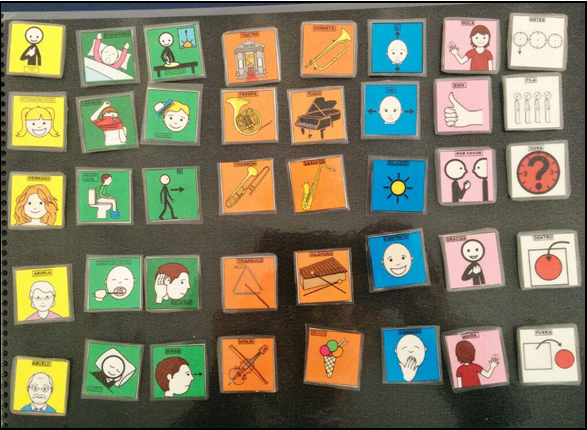
\includegraphics[width=0.7\linewidth]{Imagenes/Bitmap/tablerofisico}
	\caption{Pictographic board on which the user indicates what to communicate.}
	\label{fig:physicalboard}
\end{figure}


Communication boards are often created by teachers, parents or tutors to be used by a person with language difficulties. Traditionally they were made by cutting out and pasting pictograms on cardboard, but over time technological solutions have been implemented to facilitate this task. 

There are a multitude of applications that allow the creation of material based on pictograms, but they are generally limited to a specific format and offer little freedom to the user to create material. In addition, each of these applications has different options or facilities, such as translating a sentence into pictograms, a board where pictograms can be placed wherever you want, adding figures to the board, etc. But there is no single application that combines all these options. 
The purpose of this work is to create a web application that allows creating pictographic material quickly and easily, offering the greatest possible freedom to the user, and integrating the options most used and demanded by users in a single tool. 

\section{Objectives}
\label{cap1:sec:Objectives}



The aim of the work is to develop a web application that allows the creation of pictographic material by bringing together the functionalities most used and demanded by users. The application must have a board that allows to move with precision pictograms and other complementary elements.

For this purpose, the different existing applications will be investigated as well as the functionalities most demanded by users. Research will also be carried out into different web technologies.

Another objective is to create a simple and intuitive user interface that can be used in as many devices as possible. In order to verify the objectives of the work, an evaluation will be carried out to check the user-friendliness of the application. 


\section{Document structure}
\label{cap1:sec:mem}

The structure followed to organize this memory consists of the following chapters.
\begin{itemize}
	\item In chapter one, written in English and Spanish, it will set out the context in which the work has been carried out, also the motivation and objectives for doing so.
	
	\item Chapter two will explain briefly what a pictogram is and the different communication systems based on pictograms. In addition, the different tools related to pictograms will be discussed with an emphasis on editing communication boards.
	
	\item Chapter three will present the technologies used for the development of the application.
	
	\item Chapter four will specify the requirements and explain the created prototypes.
	
	\item Chapter five will detail the architecture and implementation of the application.
	
	\item Chapter six will show the design, results and analysis of the evaluation with users. 
	
	\item Chapter seven, written in English and Spanish, presents the final conclusions and specifies future work.
	
	\item Chapter eight will detail the tasks carried out by the two project participants.
\end{itemize}	





\end{otherlanguage}
\addtocounter{chapter}{-1} 
%%%%%%%%%%%%%%%%%%%%%%%%%%%%%%%%%%%%%%%%%%%%%%%%%%%%%%%%%%%%%%%%%%%%%%%%%%%

\chapter{Introducción}
\label{cap:introduccion}

\chapterquote{La inteligencia es la habilidad de adaptarse a los cambios}{Stephen Hawking}

\begin{resumen} En este capítulo se explicará la Motivación \ref{cap1:sec:Motivacion}, los objetivos que se quieren lograr inicialmente\ref{cap1:sec:Objetivos} y la estructura de esta memoria de TFG \ref{cap1:sec:Estructura}. 
\end{resumen}
\section{Motivación}
\label{cap1:sec:Motivacion}

Los humanos siempre hemos tenido la necesidad inherente de comunicarnos y quien no es capaz de hacerlo, generalmente acaba excluido. Y esa es la palabra clave, comunicación. Su origen proviene del latín, “\textit{communicare}”, difundir y este de “\textit{communis}” común. Gracias a ello, hemos podido llegar hasta donde estamos actualmente, una era donde todos pueden tener una voz. Por eso es más importante que nunca, no olvidarse de los que tienen dificultades. Para que puedan alzar su voz y difundir su palabra.

Sin embargo, en las últimas décadas ha habido un avance sin precedentes en el estudio e investigación sobre las discapacidades comunicativas. Éstos avances vinieron acompañados de herramientas y sistemas para facilitar la comunicación muchos de los cuales siguen vigentes a día de hoy. Uno de los principales perfiles que utilizan estos sistemas, son las  personas con trastorno del espectro autista (TEA)

Sin entrar en gran detalle, podemos encontrar que la gente con \textit{TEA} tienen dificultades en la comunicación verbal pues a menudo la comunicación no es recíproca o no se realiza en el contexto social adecuado. Respecto a la comunicación no verbal, también sufren dificultades al entender el significado de gestos faciales o expresión corporal de otras personas. Todo esto causa a menudo malentendidos, pues generalmente no se comprende el contexto y dificulta la comunicación. 

Para facilitar la comunicación se utilizan otros medios alternativos como los sistemas pictográficos, que permiten comunicarse mediante imágenes. Estos sitemas pictográficos, al estar compuestos por cientos de pictogramas habitualmente, están agrupados en \textbf{tableros pictográficos}. Estos tableros son superficies donde se colocan pictogramas para formar mensajes. Un ejemplo de tablero es el que vemos en la Figura \ref{fig:tablerofisico}. Hasta hace poco, dichos tableros eran creados a mano recortando y pegando los pictogramas pero con el tiempo se han desarrollado herramientas enfocadas a trabajar con tableros y pictogramas.

Para la elaboración de nuestra aplicación web tendremos en cuenta las aplicaciones de Pictar y PicTableros ya que ambos implementan herramientas que nos serán útiles de cara a la implementación. 

Durante este tiempo, además de estas herramientas, han surgido muchas más, cada una con sus características y funcionalidades únicas. Pero al final queda la sensación que nunca se podía hacer todo en un mismo lugar, y lo que le falta a una lo tiene otra herramienta, etc. Por ejemplo en las aplicaciones mencionadas previamente podemos ver que falta algún tipo de cuadrícula en el tablero para que a la hora de insertar los pictogramas estos queden perfectamente colocados y el tablero tenga una mejor apariencia visual.

En este contexto, la finalidad es crear una herramienta que unifique las mejores características de cada aplicación, además de permitir crear y editar tableros en un mismo lugar con la mayor facilidad posible. Afortunadamente, ya existe una base con la que nos podemos apoyar, gracias a proyectos de años anteriores como hemos mencionado, con ideas que se quedaron como trabajo futuro junto a las ideas propias. 


% TODO: \usepackage{graphicx} required
\begin{figure}[h!]
	\centering
	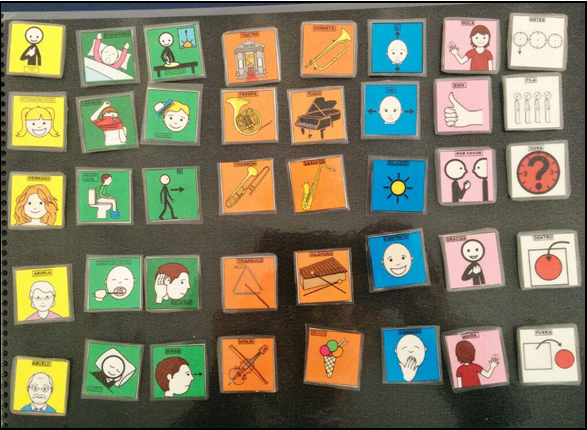
\includegraphics[width=0.7\linewidth]{Imagenes/Bitmap/tablerofisico}
	\caption{Tablero pictográfico en el que el usuario señala lo que quiere comunicar.}
	\label{fig:tablerofisico}
\end{figure}






\section{Objetivos}
\label{cap1:sec:Objetivos}

Teniendo en cuenta todos los temas que hemos tratado en la introducción queremos desarrollar una aplicación web multiplataforma que permite la edición de tableros y que incorpore una cuadrícula para ayudar a ajustar los pictogramas cuando se inserten. En la aplicación también se incorporarán herramientas de búsquedas de pictogramas por palabras y traducción de texto a pictograma.

Otro objetivo que nos hemos propuesto es que la aplicación pueda utilizarse en dos idiomas, por defecto la aplicación estará en español pero con una casilla para seleccionar el idioma se podrá cambiar a inglés. Este objetivo es sobre todo para ayudar y facilitar en el uso de esta aplicación a personas que no hablen español.

Para poder cumplir todos los objetivos mencionados se tendrá como referencia los TFG y TFM de Pictar y PicTableros. También se hará una labor de investigación en busca de nuevas tecnologías y herramientas con las que trabajar para desarrollar la aplicación. 

La forma en la que se comprobará el estado de los objetivos y su evolución será por medio de reuniones con los directores del TFG donde se analizará el trabajo realizado para ver el progreso, la forma en la que se van implementando los objetivos y la corrección de errores.



\section{Estructura de la memoria}
\label{cap1:sec:Estructura}

La estructura para memoria se encuentra dividida en [x] capítulos, a continuación se explicará brevemente su contenido. --según avancemos habrá que ir completándolo--
\begin{itemize}
	\item En los capítulos 1 y 2, se expondrá el contexto bajo el cual se ha realizado el trabajo junto a la motivación y objetivos para realizarlo.
	\item En el capítulo 3 se explicará qué es un pictograma y los distintos sistemas de comunicación con ellos. Además se analizarán las distintas herramientas relacionadas con pictogramas haciendo énfasis en la edición de tableros.
\end{itemize}	





\chapter{Estado de la Cuestión}
\label{cap:estadoDeLaCuestion}



\begin{resumen} En este capítulo se dará una idea general sobre los Sistemas aumentativos y alternativos de comunicación \ref{cap3:sec:saac}, las características de los pictogramas y los distintos sistemas pictográficos que existen \ref{cap3:sec:pictogramas}. Finalmente, se verán las distintos herramientas con las que se construyen tableros de pictogramas \ref{cap3:sec:editor-tableros}.

\end{resumen}


Los humanos siempre  han tenido la necesidad inherente de comunicarse y quien no es capaz de hacerlo generalmente acaba excluido. A día de hoy este problema sigue afectando a parte de la población como es el caso de las personas con Trastorno del Espectro Autista (\textit{TEA}).
\\

Sin entrar en gran detalle, podemos encontrar que la gente con \textit{TEA} tiene dificultades en la comunicación verbal, pues a menudo ésta no es recíproca o no se realiza en el contexto social adecuado. Respecto a la comunicación no verbal, también sufren dificultades al entender el significado de gestos faciales o expresión corporal de otras personas. Todo esto causa a menudo malentendidos, pues generalmente no se comprende el contexto y dificulta la comunicación. 


\section{Sistemas Aumentativos y Alternativos de Comunicación}
\label{cap3:sec:saac}
Los Sistemas Aumentativos y Alternativos de Comunicación (\textit{SAAC}) son las distintas formas de expresión sin tener en cuenta el lenguaje hablado que tiene como finalidad aumentar y/o compensar los problemas de comunicación de personas con discapacidad como por ejemplo trastornos del espectro autista, discapacidad intelectual, deficiencia auditiva, parálisis cerebral entre otros.

En ocasiones puede hacer falta el uso de recursos para poder comunicarse, es por ello que podemos distinguir dos tipos de \textit{SAAC}, los sistemas sin ayuda y los sistemas con ayuda.
\newpage
\begin{itemize}
	\item \textbf{Sistemas sin ayuda}: no utilizan ningún recurso externo para establecer la comunicación, únicamente usan su propio cuerpo. En los sistemas sin ayuda podemos observar dos tipos de grupos, los métodos gestuales (lengua de signos) y los métodos oralistas (lectura labiofacial). 
	\item \textbf{Sistemas con ayuda}: utilizan recursos externos para establecer la comunicación. Los más utilizados suelen ser pictogramas, imágenes o símbolos.
\end{itemize}

Las \textit{SAAC} utilizan múltiples recursos para poder comunicarse con personas con discapacidades cognitivas y entre todos ellos destacan los sistemas pictográficos. Se trata de uno de los sistemas más utilizados y esto es debido a su fácil comprensión ya que representan gráficamente lo que se desea transmitir como palabras o conceptos. 

\section{Pictogramas}
\label{cap3:sec:pictogramas}
Los pictogramas son imágenes o símbolos de rápida comprensión que expresan acciones, objetos, emociones, etc. Un conjunto de pictogramas en un cierto orden, pueden generar una oración. Todos ellos deben cumplir las siguientes características\footnote{\url{http://aularagon.catedu.es/materialesaularagon2013/arasaac/ZIPs/Modulo_1/contenidos.html}}:
\begin{enumerate}
	\item \textbf{Referencialidad}: relación del pictograma con el referente.
	\item \textbf{Ítems gráficos}: imágenes que representen de manera sencilla aquello que se toma como modelo.
	\item \textbf{Comprensión}: debe ser fácilmente entendible independientemente de la formación, idioma o discapacidad.
	\item \textbf{Legibilidad}: mantener una coherencia visual entre pictogramas.
	\item \textbf{Sencillez}: mostrar únicamente los elementos relevantes sin elementos distractores o adornos insignificantes.
\end{enumerate}


 
Existen numerosos sistemas pictográficos. A continuación hablaremos de algunos de los más relevantes:

\subsection{Sistema Pictográfico de Comunicación - SPC}

El Sistema Pictográfico de Comunicación\footnote{\url{https://www.uv.es/bellochc/logopedia/NRTLogo8.wiki?8}} (\textit{SPC}) fue creado en 1981 por Roxana Mayer Johnson, con la intención de facilitar la comunicación a quienes tienen un nivel de lenguaje expresivo simple o vocabulario limitado. Gracias a la diferenciación por colores, facilita la comprensión de la estructura sintáctica. Actualmente cuenta con más de 3000 iconos. Está organizado por seis colores según su función gramatical como podemos ver en la Figura \ref{fig:spccolores}.

\begin{itemize}
	\item \textbf{Personas} (Amarillo): representan a familiares y pronombres. Ejemplo: mamá, familia,  yo, ellos.
	\item \textbf{Verbos} (Verde): representan acciones. Ejemplo: abrir, agarrar, comer, ir.
	\item \textbf{Descriptivos} (Azul): representan descripciones, adjetivos y adverbios. Ejemplo: bonito, triste, vacío, lleno.
	\item \textbf{Nombre} (Naranja): representan objetos u otros elementos que no aparecen en otra categoría. Ejemplo: gato, almohada o casa.
	\item \textbf{Miscelánea} (Blanco): representa números, letras y colores
	\item \textbf{Social} (Rosa): vocabulario relacionado con relaciones sociales. Ejemplo: buenos días, sí, gracias, no lo sé.
	
\end{itemize}

% TODO: \usepackage{graphicx} required
\begin{figure}[h!]
	\centering
	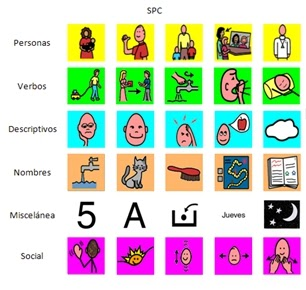
\includegraphics[width=0.7\linewidth]{Imagenes/Bitmap/SPCcolores}
	\caption{Ejemplo de categorías en SPC.}
	\label{fig:spccolores}
\end{figure}

\subsection{Blissymbolics}
Byssimbolics\footnote{\url{https://www.blissymbolics.org/index.php/about-blissymbolics}}
es un sistema de comunicación que fue usado por primera vez en 1971 para facilitar la comunicación con niños que padecían alguna discapacidad. Actualmente está compuesto por más de 5000 símbolos o  \textit{Bliss-Words} los cuales a su vez están compuestos por uno o más Caracteres-Bliss o  \textit{Bliss-Characters}. A pesar de que los 150 \textit{Bliss-Characters} que hay son sencillos de dibujar, requieren un periodo de aprendizaje para comprender su significado y así el de las \textit{Bliss-Words}. En la Figura \ref{fig:blisscharacters} vemos algunos \textit{Bliss-Characters} con su significado. \\
% TODO: \usepackage{graphicx} required

\begin{figure}[h!]
	\centering
	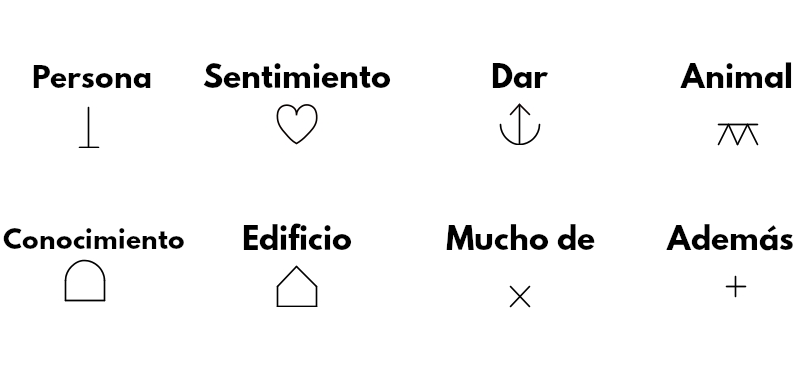
\includegraphics[width=0.8\linewidth]{Imagenes/Bitmap/BlissCharacters}
	\caption[Ejemplo de Bliss-Characters]{Ejemplo de Bliss-Characters.}
	\label{fig:blisscharacters}
\end{figure}
Una vez comprendido, en la Figura \ref{fig:blissword} vemos cómo se han combinado para generar \textit{Bliss-Words}. Destacar que el orden, el tamaño o la posición de los los Bliss-Characters, puede alterar su significado. Adicionalmente pueden estar agrupados de los mismos colores vistos en SPC.

% TODO: \usepackage{graphicx} required
\begin{figure}[h!]
	\centering
	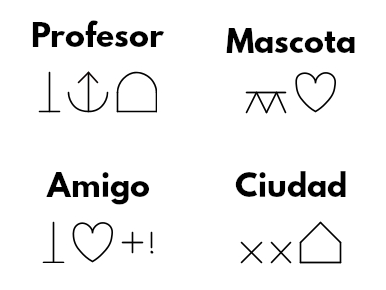
\includegraphics[width=0.4\linewidth]{Imagenes/Bitmap/BlissWord}
	\caption[Ejemplo de Bliss-Words]{Ejemplo de Bliss-Words.}
	\label{fig:blissword}
\end{figure}



\subsection{Sclera}
La principal característica de Sclera\footnote{\url{https://www.sclera.be/en/picto/overview}} frente a otros sistemas pictográficos es que sus pictogramas son menos coloridos pero cuentan con pictogramas más avanzados en cuanto a acciones representadas. Un ejemplo de ello se puede ver en la Figura \ref{fig:sclera} donde la acción de pedir atención se puede realizar de dos maneras posibles. Cuenta con un total de 11.497 pictogramas en español.

En la actualidad el desarrollo de Sclera está paralizado desde 2015.



% TODO: \usepackage{graphicx} required
\begin{figure}[h!]
	\centering
	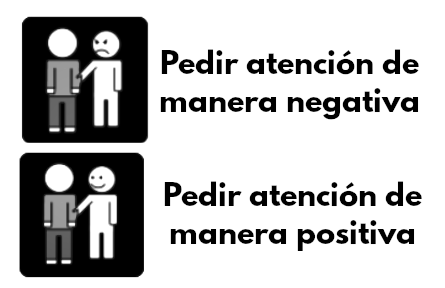
\includegraphics[scale=0.5]{Imagenes/Bitmap/Sclera}
	\caption{Ejemplo de acciones en Sclera.}
	\label{fig:sclera}
\end{figure}

\newpage
\subsection{Mulberry Symbols}
Mulbery Symbols\footnote{\url{https://mulberrysymbols.org/}} se creó con el propósito de ser un sistema pictográfico orientado a adultos ya que un gran porcentaje de dichos sistemas estaban pensados principalmente para niños y dificultaban la comunicación por falta de pictogramas. Como se observa en la Figura \ref{fig:mulberry} podemos ver ejemplos de pictogramas enfocados a adultos como cerveza o fumar.

Todos los pictogramas se pueden descargar gratuitamente desde su página web en formato ZIP cuyas imágenes se encuentran en formato SVG o en formato CSV donde están categorizados según su nombre y categoría. 
Los pictogramas de Mulbery cuentan con 118 categorías incluyendo sustantivos, pronombres, verbos sumando un total de 3.436 pictogramas. A diferencia de otros sistemas pictográficos Mulbery sigue en activo añadiendo constantemente nuevos pictogramas. 

Los pictogramas de Mulbery son utilizados por muchas aplicaciones como BoradBuilder\footnote{\url{ https://globalsymbols.com/boardbuilder/boardsets}} (aplicación web para diseñar tableros de comunicación), Cboard\footnote{\url{https://www.cboard.io/}} (aplicación web de comunicación que usa pictogramas y conversión de texto a voz) o CommuniKate\footnote{\url{http://communikate.equalitytime.co.uk/}} (página web que ofrece tableros diseñados en Powerpoint o Impress). Una de las últimas herramientas creadas que hace uso de los pictogramas de Mulbery es la diseñada por Eliada Pampoulou y Maria Constanta de la Universidad Tecnológica de Chipre la cual usa unas plantillas imprimibles en inglés\footnote{\url{https://mulberrysymbols.org/assets/COVID19/Covid-19_AAC-EN.pdf}} o griego para ayudar a la comunicación de los pacientes con la COVID-19 que tienen dificultades para comunicarse.



% TODO: \usepackage{graphicx} required
\begin{figure}[h!]
	\centering
	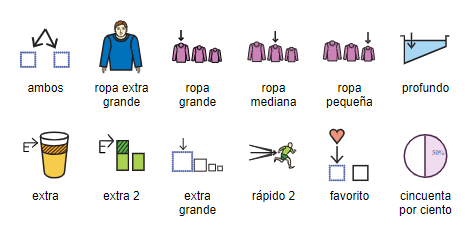
\includegraphics[scale=0.2]{Imagenes/Bitmap/Mulberry}
	\caption{Ejemplo de pictogramas de Mulberry.}
	\label{fig:mulberry}
\end{figure}

\newpage
\subsection{Minspeak}
Minspeak\footnote{\url{http://ares.cnice.mec.es/informes/18/contenidos/94.htm}}. es un sistema de comunicación alternativo creado por Bruce Baker en 1982. Difiere con los vistos anteriormente en que el significado de los iconos no viene preestablecido sino que es acordado entre usuario y logopeda. Es por ello que cada icono acordado tenga un significado distinto según la secuenciación de iconos. Por ejemplo en el caso de la Figura \ref{fig:minspeak} la asociación del icono casa junto a la cama, en ese orden podría ser interpretado como dormitorio. 

% TODO: \usepackage{graphicx} required
\begin{figure}[h!]
	\centering
	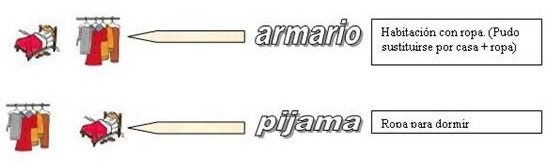
\includegraphics[width=0.7\linewidth]{Imagenes/Bitmap/Minspeak}
	\caption{Ejemplo de Minspeak.}
	\label{fig:minspeak}
\end{figure}

Como cada pictograma puede tener un significado distinto según su orden, se crearon Programas de Comunicación Minspeak (\textit{PAM}). Éstos se usan para cuando una casilla o icono haya sido seleccionada, se activen los posibles iconos con los que pueda tener algún tipo de relación. Inicialmente se creó hardware específico como aparece en la Figura \ref{fig:chatbox} con 16 celdas las cuales podía generar hasta 1024 mensajes, los teclados evolucionaron con más celdas y combinaciones, hasta pasar a teclados digitales implementados por software como PortaVoz\footnote{\url{http://www.terapia-ocupacional.com/articulos/Portavoz_JMLedesma.shtml}}.

% TODO: \usepackage{graphicx} required
\begin{figure}[h!]
	\centering
	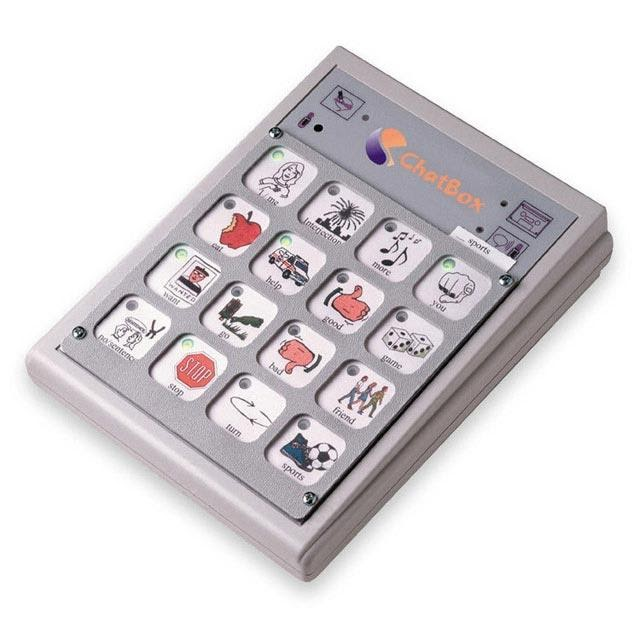
\includegraphics[width=0.4\linewidth]{Imagenes/Bitmap/ChatBox}
	\caption[ChatBox]{Panel de ChatBox}
	\label{fig:chatbox}
\end{figure}



\subsection{ARASAAC}

El portal Aragonés de Comunicación Aumentativa y Alternativa \\ \textit{ARASAAC}\footnote{\url{http://www.arasaac.org/}}
 surge en 2007 gracias a la colaboración entre el personal del CATEDU, el colegio público de educación Especial Alborada y del Centro Politécnico Superior de la Universidad de Zaragoza. Su objetivo era la creación de un sistema pictográfico de libre distribución que ayudara en el ámbito de la comunicación a todas aquellas personas que lo necesitasen.
Actualmente el portal de \textit{ARASAAC} incluye fotografias, videos y cuenta con más de 39000 pictogramas tanto a color como en blanco y negro y con traducciones a 20 idiomas. También ofrece herramientas online con las que poder generar materiales como por ejemplo generador de calendarios, generador de tableros, creador de símbolos, etc.

A diferencia de otros sistemas pictográficos, \textit{ARASAAC} permite una gran cantidad de opciones configurables como el color de fondo, marco o tiempo verbal, la Figura \ref{fig:configuarcion-arasaac} muestra todas las posibles opciones de configuración.



\begin{figure}[h!]
	\centering
	\includegraphics[width=0.7\linewidth]{Imagenes/Bitmap/Configuarción ARASAAC}
	\caption{Opciones de configuración de un pictograma.}
	\label{fig:configuarcion-arasaac}
\end{figure}



En la actualidad \textit{ARASAAC} es uno de los sistemas pictográficos más utilizados a nivel de educación especial en España. Sus pictogramas se utilizan en colegios, universidades e incluso se han creado asociaciones para facilitar su implantación. CreaTea es una asociación en la Comunidad de Madrid cuyo objetivo es habilitar lugares como clínicas, restaurantes o ayuntamientos, para ayudar a la inclusión de personas con dificultades en la comunicación y concienciar a la sociedad.

También cabe destacar que \textit{ARASAAC} ha recibido varios premios por su labor y que es una herramienta utilizada en varios países por lo que la cantidad de usuarios que colaboran es muy alta. Esto queda reflejado en la cantidad de pictogramas que se publican a la plataforma por parte de colaboradores sin ánimo de lucro y dichos pictogramas están constantemente actualizándose. Un ejemplo de ellos son los pictogramas que se han publicado debido a la pandemia como por ejemplo las Figuras \ref{fig:picto-mascarilla} y \ref{fig:picto-mascarilla-mal-colocada}.

\newpage
% TODO: \usepackage{graphicx} required
\begin{figure}[h!]
	\centering
	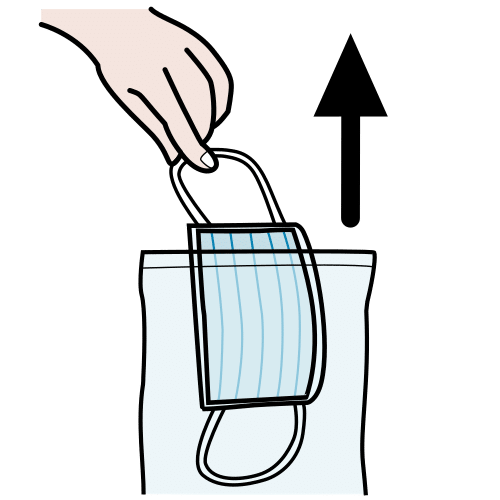
\includegraphics[width=0.2\linewidth]{Imagenes/Bitmap/Picto Mascarilla}
	\caption{Acción de sacar la mascarilla.}
	\label{fig:picto-mascarilla}
\end{figure}

\begin{figure}[h!]
	\centering
	
\includegraphics[width=0.2\linewidth]{Imagenes/Bitmap/Mascarilla mal colocada}
	\caption{Pictograma que representa mascarilla mal colocada.}
	\label{fig:picto-mascarilla-mal-colocada}
\end{figure}

En la Figura \ref{fig:arasaacpictos} podemos ver algunos ejemplos de pictogramas de \textbf{ARASAAC} en situaciones o casos más cotidianos. Destacan la manera clara y concisa en la que están representados. 

% TODO: \usepackage{graphicx} required
\begin{figure}[h!]
	\centering
	
\includegraphics[width=0.7\linewidth]{Imagenes/Bitmap/ARASAACPictos}
	\caption{Ejemplo de pictogramas más típicos de \textit{ARASAAC}.}
	\label{fig:arasaacpictos}
\end{figure}

La licencia de \textit{ARASAAC} es de tipo \textit{Creative Commons (BY-NC-SA)} por lo que se podrá utilizar el material elaborado por ellos de cara a la implementación del Trabajo Fin de Grado. Utilizaremos sus pictogramas publicados en su página web y la API que han desarrollado para acceder a pictogramas de su base de datos.

\section{Editores de Tableros basados en Pictogramas}
\label{cap3:sec:editor-tableros}

Ya hemos visto multitud de sistemas pictográficos, pero para trabajar con ellos es necesario que sean fáciles de acceder, pues es fácil encontrar cientos de pictogramas en cada sistema pictográfico. La solución a esto, son los tableros pictográficos. Los tableros son un área en la que se pueden colocar pictogramas, fotografías o palabras que la persona indicará para comunicarse. Pueden tener distintas funciones, como por ejemplo hacer un horario, normas, o elegir entre distintas opciones mediante pictogramas. A menudo estos tableros se realizan mediante piezas de papel recortadas, como podemos ver en la Figura \ref{fig:editorespictogramas}.

% TODO: \usepackage{graphicx} required
\begin{figure}[h!]
	\centering
	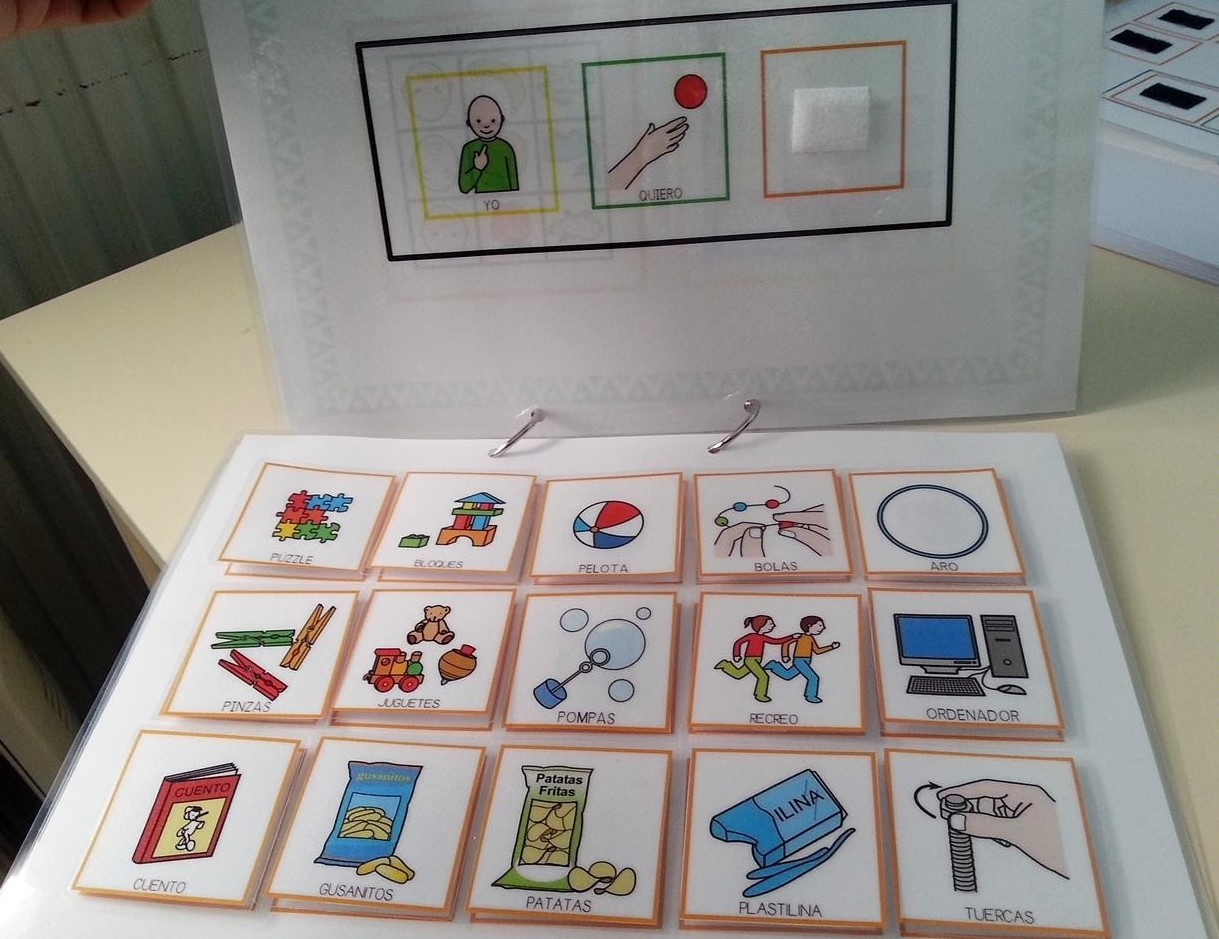
\includegraphics[width=0.7\linewidth]{Imagenes/Bitmap/EditoresPictogramas}
	\caption{Ejemplo de tablero para pictogramas en papel.}
	\label{fig:editorespictogramas}
\end{figure}

Estos tableros\footnote{\url{http://burbujadelenguaje.blogspot.com/2016/05/tablero-de-comunicacion-tea.html}}, no tienen por qué limitarse a un espacio rectangular, sino que se pueden usar de maneras más creativas dependiendo de las discapacidades de la persona que lo use. Por ejemplo los \textit{ETRAN}\footnote{\url{http://psicosociosanitario.blogspot.com/2016/05/tableros-de-comunicacion.html}}. (“Eye-Transfer”) son usados por gente con baja movilidad y que apuntan al pictograma con la mirada, otra persona está al otro lado del \textit{ETRAN} para ver qué pictograma está mirando como podemos ver en la Figura \ref{fig:tablero}. Otro ejemplo son los cuadernos de comunicación que como su nombre indica son un conjunto de hojas o tableros con símbolos básicos.

% TODO: \usepackage{graphicx} required
\begin{figure}[h!]
	\centering
	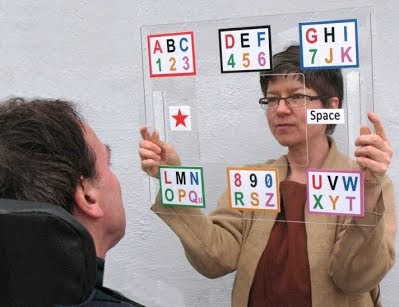
\includegraphics[width=0.7\linewidth]{Imagenes/Bitmap/Tablero}
	\caption{Uso de tablero ETRAN.}
	\label{fig:tablero}
\end{figure}

Trabajar con piezas de papel puede resultar engorroso y a menudo poco eficiente, por eso ha sufrido una evolución natural al medio digital, y con ello software de edición de tableros pictográficos. Gracias a ello, podremos ahorrar mucho trabajo, como buscar pictogramas, alinearlos, editarlos o incluso poder compartir los tableros.


Para crear y editar tableros se han creado multitud de aplicaciones, a continuación estudiaremos sus características.



\subsection{Pictoselector}
Es una herramienta gratuita para crear agendas visuales. Recopila más de 28.000 provenientes de \textbf{\textit{Sclera}}, \textbf{\textit{Mulberry}}, \textbf{\textit{ARASAAC}}, etc. Al crear un proyecto, permite cargar una plantilla o crear una desde cero. Se puede modificar el número de filas y columnas, la posición del texto y el tamaño del borde de los pictogramas.
\footnote{\url{ https://www.pictoselector.eu/es/ }}

% TODO: \usepackage{graphicx} required
\begin{figure}[h!]
	\centering
	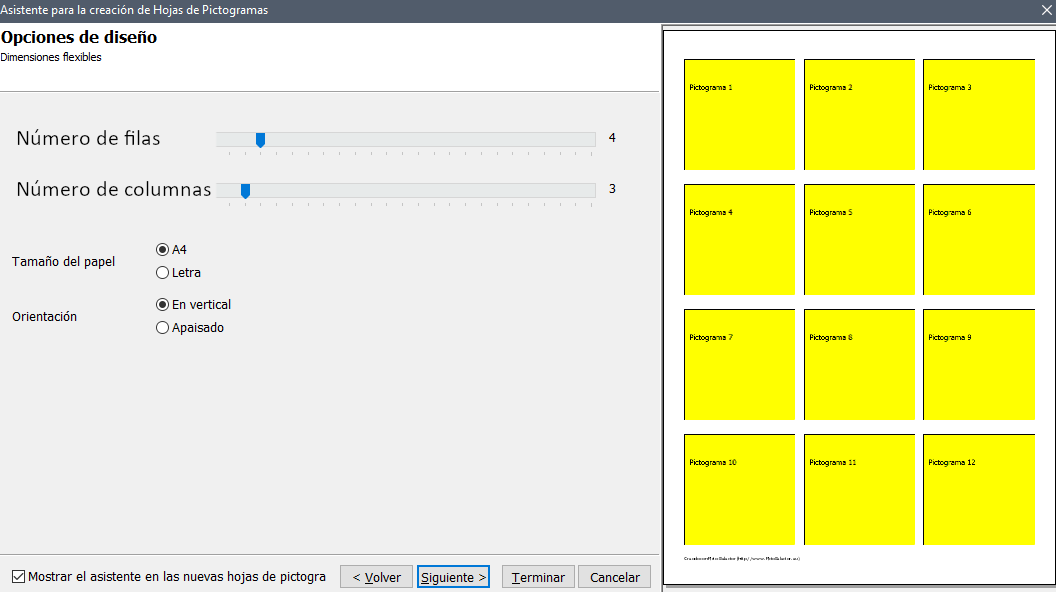
\includegraphics[width=0.7\linewidth]{Imagenes/Bitmap/Pictoselector Tablero}
	\caption{Ventana donde se edita el tamaño de la cuadrícula.}
	\label{fig:pictoselector-tablero}
\end{figure}


Una vez creado el tablero, podemos insertar en su cuadrícula distintos elementos, muchos de ellos en forma de pictograma. Para facilitar esta tarea, la cabecera de la aplicación contiene acceso directo a la inserción de pictogramas



Como podemos ver, de izquierda a derecha, existe un buscador de pictogramas que incluye la función de filtrar por juego de pictogramas. Además de poder editar ligeramente el picto ya sea coloreándolo o añadiendo un signo de pasado, presente o plural. Para el marcaje de tiempo pueden incluirse con facilidad pictogramas de reloj que marcan la hora y de duración que marcan un intervalo de tiempo. Adicionalmente se puede importar imágenes propias, códigos QR , texto o emoticonos.

% TODO: \usepackage{graphicx} required
\begin{figure}[h!]
	\centering
	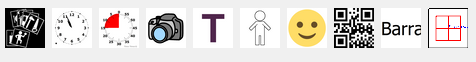
\includegraphics[width=0.7\linewidth]{Imagenes/Bitmap/Ribbon Pictoselector}
	\caption{Barra de inserción de pictogramas.}
	\label{fig:ribbon-pictoselector}
\end{figure}

% TODO: \usepackage{graphicx} required
\begin{figure}[h!]
	\centering
	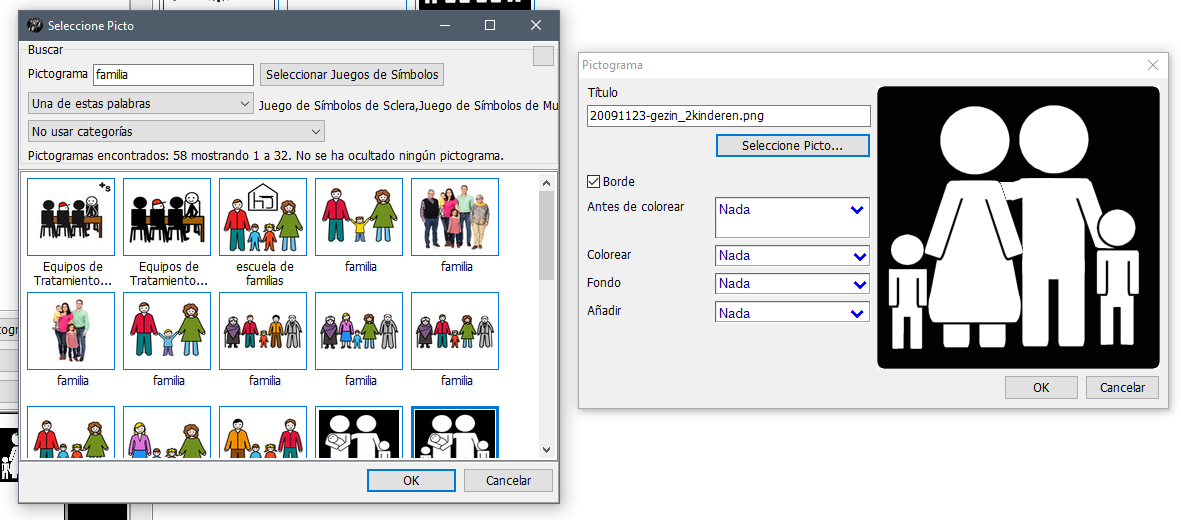
\includegraphics[width=0.7\linewidth]{Imagenes/Bitmap/Editor y buscador de pictoselector}
	\caption{Buscador y editor de Pictogramas.}
	\label{fig:editor-y-buscador-de-pictoselector}
\end{figure}




El mayor inconveniente de la aplicación, pese a ser muy completa respecto a la búsqueda y edición de pictos, es su limitación de colocación a una cuadrícula.

\subsection{Editor ARASAAC}
La página web de \textit cuenta con herramientas online las cuales podemos usar para generar materiales .
\begin{itemize}
\item \textbf{Creador de animaciones}: genera una animación con los pictogramas que queramos en formato GIF o SWF. También permite configurar el intervalo entre los pictogramas y el número de repeticiones que hará.

\item \textbf{Creador de símbolos}: permite la personalización de pictogramas donde podremos cambiar el nombre del pictograma, poner su traducción, modificar la fuente del texto, poner un marco, ampliar la imagen y cambiar el fondo.

\item \textbf{Generador de frases}: consta de un total de tres pasos a seguir, el primero de ellos consiste en seleccionar las palabras que queramos traducir a pictogramas, el segundo paso nos mostrará todos los pictogramas asociados para cada palabra introducida y deberemos seleccionar el que más nos guste y el tercer paso aparecerán todos los pictogramas colocados en una tabla la cual podremos modificar.
\footnote{\url{ http://www.arasaac.org/herramientas.php }}

% TODO: \usepackage{graphicx} required
\begin{figure}[h!]
	\centering
	
\includegraphics[width=0.7\linewidth]{Imagenes/Bitmap/Frase ARASAAC}
	\caption{Ejemplo con generador de frases.}
	\label{fig:frase-arasaac}
\end{figure}


\item \textbf{Generador de horarios}: genera un horario donde previamente tendremos que configurar una plantilla con los días, horas, el formato (horizontal o vertical), idioma, bordes del horario, texto para cada día y hora y la opción de insertar un pictograma en función de su día y hora.

\item \textbf{Generador de calendarios}: genera un calendario donde tendremos que especificar el mes, año e idioma deseado. Al igual que en el generador de horarios permite la opción de modificar el texto, colores, bordes y la posibilidad de poner un pictograma para cada día del mes.

\item \textbf{Generador de tableros}: crea un tablero con el número de filas y columnas deseado donde para cada casilla podremos insertar un pictograma. Al igual que en otras herramientas permite la modificación de colores, bordes y  texto del tablero.

\item \textbf{Creador de juegos}: genera una plantilla en formato .rtf para poder jugar al bingo, oca, dominós y dominós encadenados con los pictogramas que deseemos.
\end{itemize}

% TODO: \usepackage{graphicx} required
\begin{figure}[h!]
	\centering
	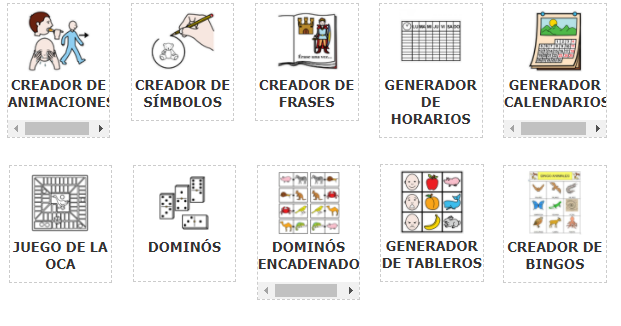
\includegraphics[width=0.4\linewidth]{Imagenes/Bitmap/Tableros ARASAAC}
	\caption[Tableros web ARASAAC]{Herramientas online que ofrece ARASAAC.}
	\label{fig:tableros-arasaac}
\end{figure}

\newpage
\subsection{Piktoplus}
Se trata de una aplicación para dispositivos Android. Su particularidad es que permite la creación de un avatar tridimensional personalizable\footnote{\url{http://www.aulautista.com/2013/12/05/piktoplus-un-comunicador-android-muy-especial/ }}. Dicho avatar será usado en los tableros pictográficos pues será quien protagonice las acciones. Permite registrar múltiples usuarios, cada uno con su propio avatar. Otra particularidad de Piktoplus son los sub-tableros. \footnote{\url{https://fatimamikel.wordpress.com/2014/04/17/piktoplus-2/ }}  Por ejemplo, en la Figura \ref{fig:piktoplus1}  hay un tablero con dos pictogramas, “Estoy” y “Me duele”.


% TODO: \usepackage{graphicx} required
\begin{figure}[h!]
	\centering
	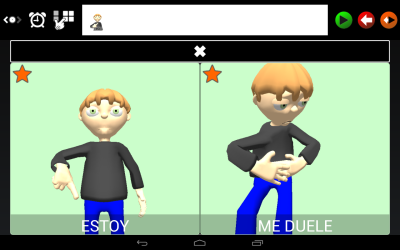
\includegraphics[width=0.5\linewidth]{Imagenes/Bitmap/Piktoplus1}
	\caption[Pictoplus tablero]{Ejemplo de tablero en Piktoplus}
	\label{fig:piktoplus1}
\end{figure}

En el caso que pusemos sobre estoy, se desplegará un sub-tablero dentro del mismo tablero con cuatro pictogramas como se representa en la Figura \ref{fig:piktoplus2}.


% TODO: \usepackage{graphicx} required
\begin{figure}[h!]
	\centering
	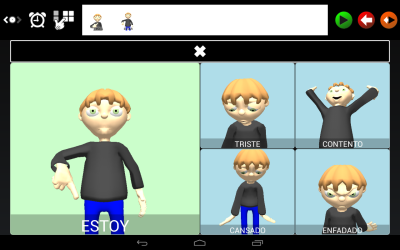
\includegraphics[width=0.5\linewidth]{Imagenes/Bitmap/Piktoplus2}
	\caption[Subtablero Piktoplus]{Subtablero en Piktoplus}
	\label{fig:piktoplus2}
\end{figure}


Respecto a la creación y edición de tableros, se trata de una cuadrícula sobre la cual se colocan los pictogramas, además permite aumentar el tamaño de los pictos. Por ejemplo “Estoy” ocupa cuatro celdas más que “Contento”. 

Actualmente esta aplicación no está disponible para descargar en tiendas de aplicaciones  habituales y su desarrollo ha cesado desde 2018. Aunque no esté disponible, plantea una idea muy interesante como la posibilidad de desplegar un sub-tablero a partir de un pictograma para mostrar pictogramas relacionados entre ellos.

\subsection{BoardMaker}
VER A FINALES DE MES PARA UNA POSIBLE ACTUALIZACIÓN DE APP

\subsection{Pictar}
Pictar\footnote{\url{ http://hypatia.fdi.ucm.es/pictar/}} es una aplicación web desarrollada por el alumno Alejandro Martín Guerrero de la Universidad Complutense de Madrid del grado de ingeniería informática como Trabajo de Fin de Máster. El propósito de Pictar es poder tener una aplicación web accesible desde cualquier dispositivo con conexión a internet para facilitar la comunicación a personas con TEA.

Pictar ofrece tres herramientas en su página web:
\begin{itemize}
	\item \textbf{Traducir frase}:permite generar una secuencia de pictogramas asociados a una frase o texto introducido por el usuario. Ofrece la posibilidad tras haber generado la secuencia de pictogramas, de poder cambiarlos por otros pictogramas del mismo significado mediante unas flechas que se encuentran tanto encima como debajo de cada pictograma. También incluye un icono que tiene como finalidad copiar la secuencia de pictogramas generados al tablero, ver la Figura \ref{fig:traducirfrase}.
	
	% TODO: \usepackage{graphicx} required
	\begin{figure}[h!]
		\centering
		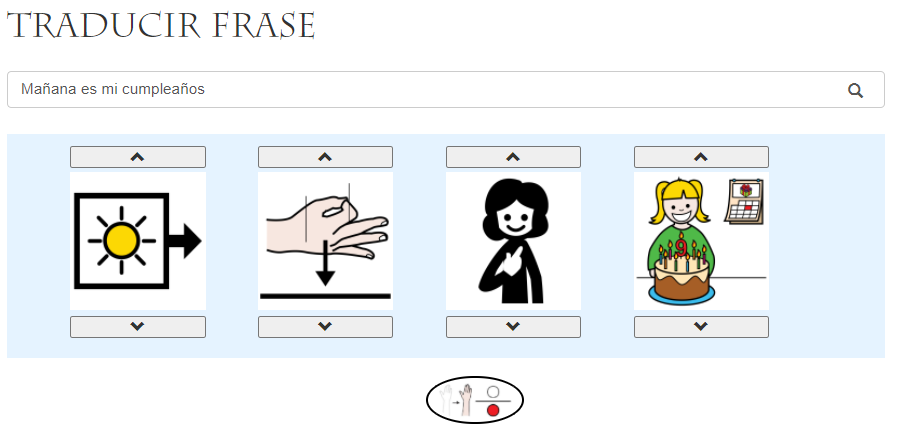
\includegraphics[width=0.7\linewidth]{Imagenes/Bitmap/TraducirFrase}
		\caption{Funcionalidad en la aplicación Pictar de traducir frase.}
		\label{fig:traducirfrase}
	\end{figure}

	\item \textbf{Buscador}: al introducir una palabra en el campo de búsqueda nos mostrará todos aquellos pictogramas con un significado igual o similar a la palabra introducida, ejemplo de ello en la Figura \ref{fig:buscador}. El buscador ofrece la posibilidad de poder arrastrar los pictogramas para insertarlos al tablero que se muestra en la Figura \ref{fig:editor}.
	
	% TODO: \usepackage{graphicx} required
	\begin{figure}[h!]
		\centering
		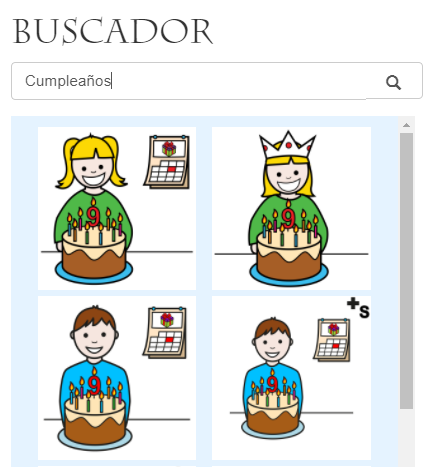
\includegraphics[width=0.5\linewidth]{Imagenes/Bitmap/buscador}
		\caption{Funcionalidad en la aplicación Pictar de buscador.}
		\label{fig:buscador}
	\end{figure}
	
	
	\item \textbf{Editor}: permite generar un tablero de pictogramas en el que deberemos seleccionar cuantos elementos va a tener en total y el número de columnas en los que se divide. Para añadir pictogramas al tablero tenemos dos opciones: la primera de ella es copiar la secuencia generada al traducir una frase a pictogramas y la segunda buscar un pictograma en el buscador para poder arrastrar el pictograma deseado al tablero. Por cada pictograma insertado en el tablero tendremos dos opciones debajo de éste situadas en las esquinas inferiores izquierda y derecha que permiten eliminar o dejar la casilla en blanco. El editor ofrece la posibilidad de añadir el nombre a cada pictograma, poner todos los pictogramas a color o blanco y negro y exportar o importar el tablero. Todas estas características se pueden observar en la Figura \ref{fig:editor}.
	
	% TODO: \usepackage{graphicx} required
	\begin{figure}[h!]
		\centering
		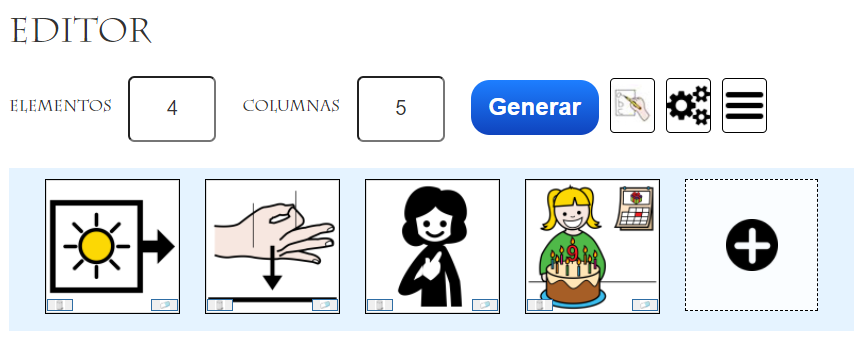
\includegraphics[width=0.7\linewidth]{Imagenes/Bitmap/editor}
		\caption{Funcionalidad en la aplicación Pictar de editor.}
		\label{fig:editor}
	\end{figure}
	
	
\end{itemize}




\newpage
\subsection{Pictableros}
\footnote{\url{ https://holstein.fdi.ucm.es/picto-tableros/  }}
Pictableros es una aplicación web de edición y creación de tableros y plantillas para pictogramas. Tiene dos partes diferenciadas:

\begin{itemize}
	\item Las plantillas sirven para que otros usuarios que quieran crear un tablero similar puedan sustituir con facilidad los pictogramas. Por ejemplo en la Figura \ref{fig:pictableros1} existe una plantilla de tablero para elegir un deporte, dicha plantilla puede ser modificada para sustituir el pictograma de balonmano por tenis. Estas plantillas pueden ser públicas o privadas.
	
	\item Los tableros públicos no pueden ser modificados, aunque  se puede crear una copia de ellos y modificarse para superponer símbolos (Bien, mal, amarillo, azul)
	

\end{itemize}

	% TODO: \usepackage{graphicx} required
	\begin{figure}[h!]
		\centering
		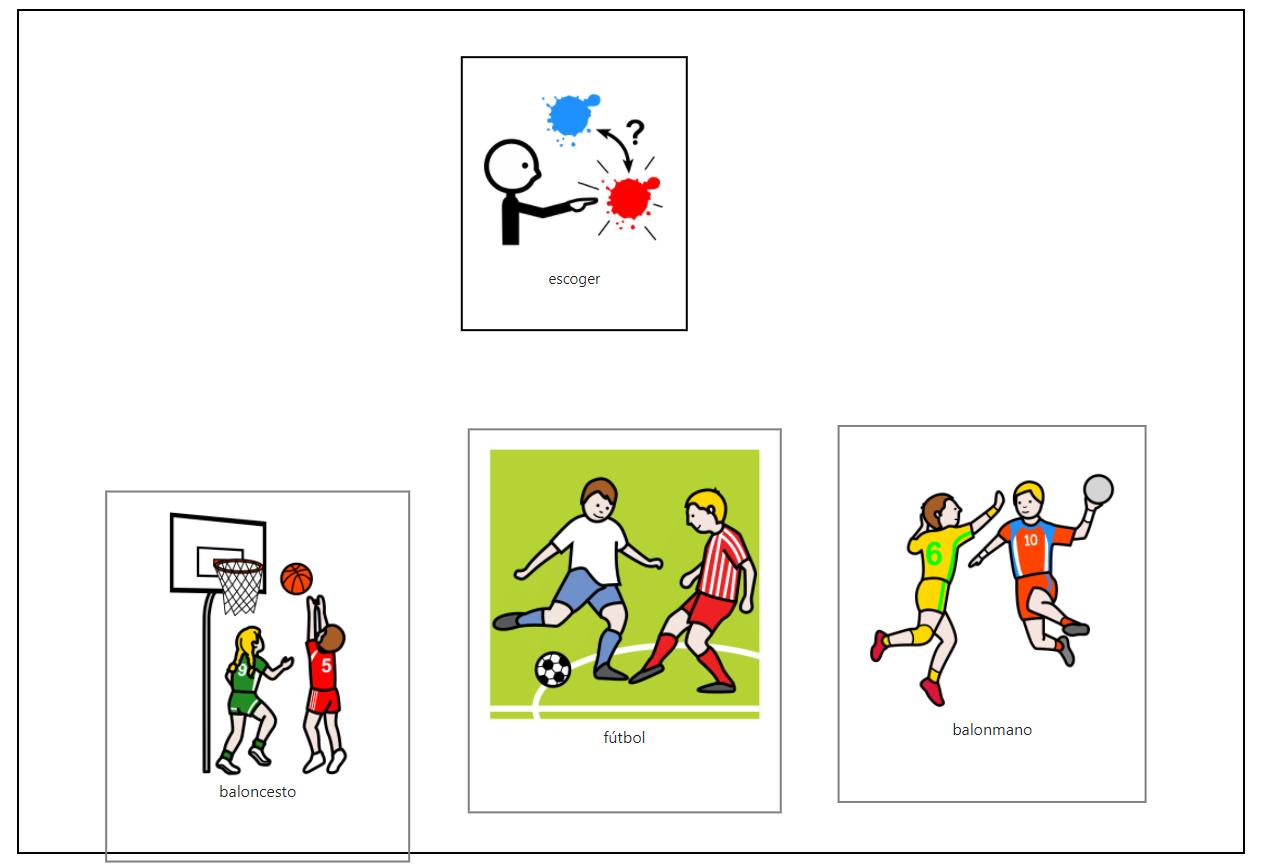
\includegraphics[width=0.7\linewidth]{Imagenes/Bitmap/pictableros1}
		\caption{Plantilla de elección de deporte.}
		\label{fig:pictableros1}
	\end{figure}
	
	
	% TODO: \usepackage{graphicx} required
	\begin{figure}[h!]
		\centering
		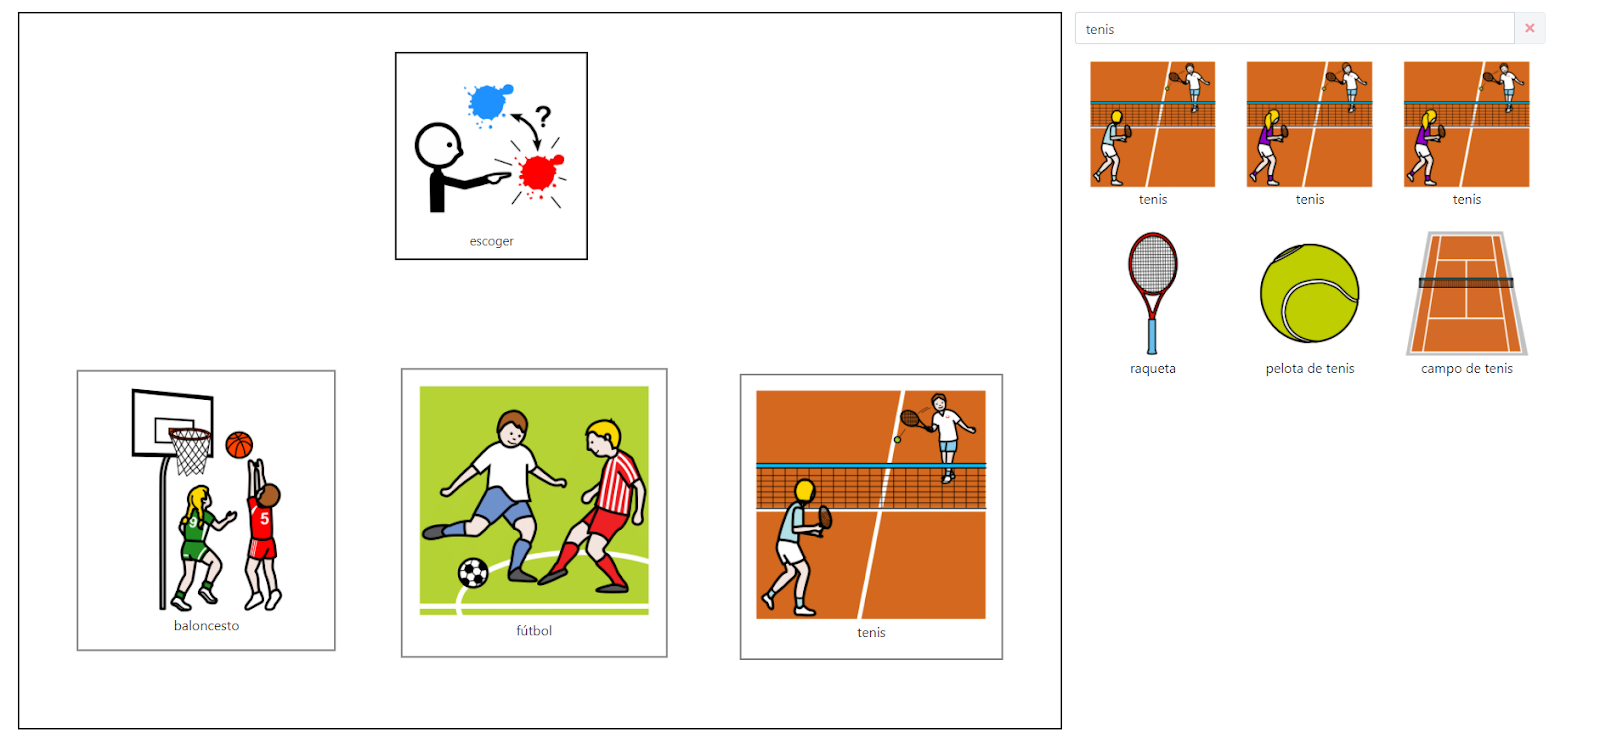
\includegraphics[width=0.7\linewidth]{Imagenes/Bitmap/pictableros2}
		\caption[Edición de plantilla en Pictableros]{Edición de plantilla de selección de deporte, sustituimos balonmano por tenis, haciendo uso del buscador de pictogrmas.}
		\label{fig:pictableros2}
	\end{figure}
	
	% TODO: \usepackage{graphicx} required
	\begin{figure}[h!]
		\centering
		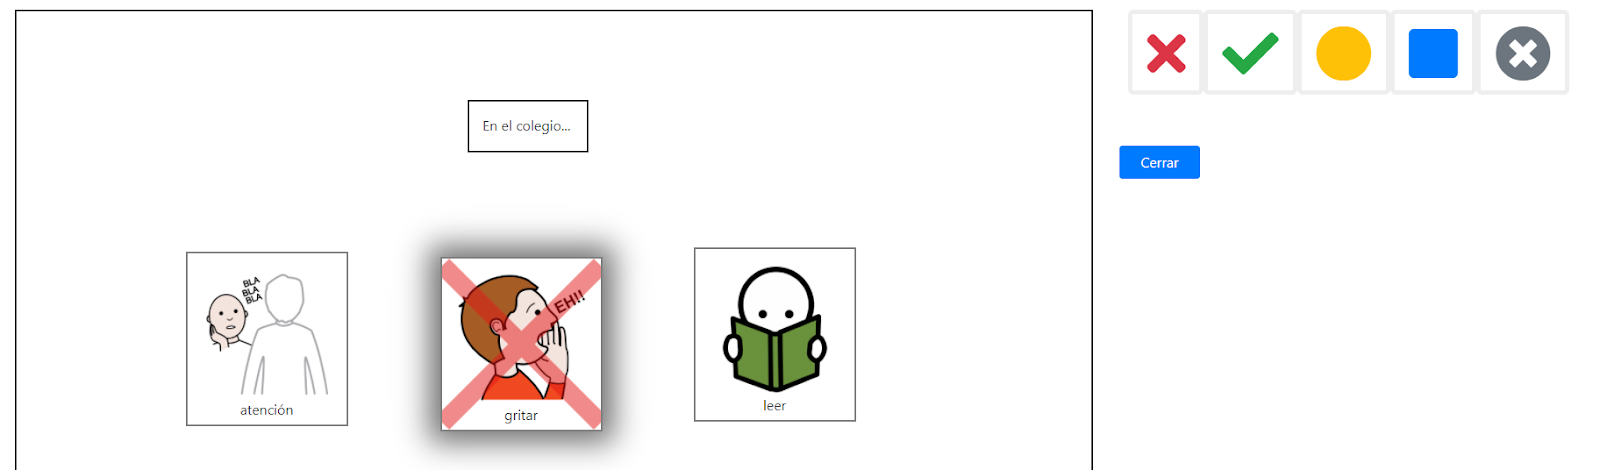
\includegraphics[width=0.7\linewidth]{Imagenes/Bitmap/pictableros3}
		\caption[Edición plantilla en Pictableros]{Edición de tableros, permite superponer un signo al pictograma.}
		\label{fig:pictableros3}
	\end{figure}
	

	


\newpage	
\subsection{Symbo Talk}

SymboTalk permite la creación de tableros de comunicación aumentativa y locución de tableros y pictogramas mediante su aplicación web o dispositivos móviles como Android e iOS.
\footnote{\url{  https://civat.es/app/symbo-talk/ }}
\footnote{\url{   http://aulaabierta.arasaac.org/symbotalk-0-inicio-2  }}
SymboTalk ofrece dos modos de usuario:

\begin{itemize}
	\item \textbf{Modo edición}: permite la creación de pictogramas, construir tableros, buscar pictogramas en un buscador. También ofrece la opción de crear un perfil y poder guardar todos los tableros que hayamos realizado.
	
	\item \textbf{Modo usuario}: pensado para que el usuario pueda comunicarse de una forma más fácil e intuitiva.
	
\end{itemize}

% TODO: \usepackage{graphicx} required
\begin{figure}[h!]
	\centering
	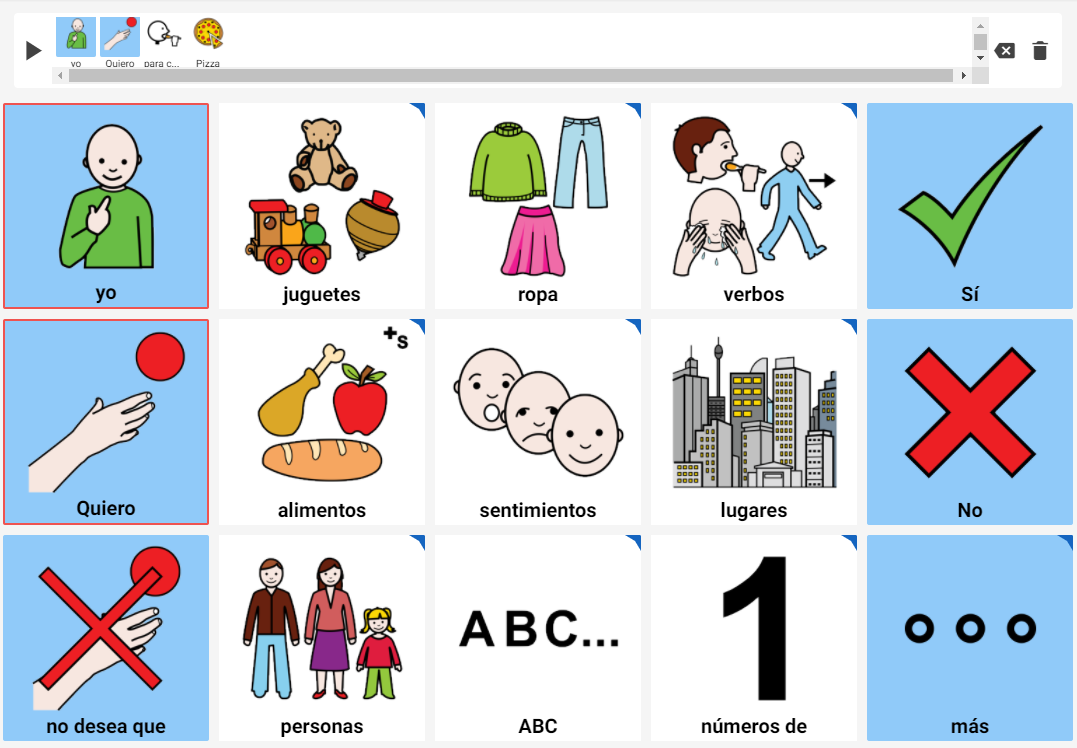
\includegraphics[width=0.7\linewidth]{Imagenes/Bitmap/SymboTalk}
	\caption{Pantalla principal de la aplicación Symbo Talk.}
	\label{fig:symbotalk}
\end{figure}

\newpage
\subsection{LetMe Talk}

LetMe Talk es una aplicación para dispositivos Android e iOS que permite generar frases a partir de pictogramas seleccionados. Tiene un total de 9.000 pictogramas de \textit{ARASAAC} y ofrece la posibilidad de añadir imágenes con un texto descriptivo con la cámara del dispositivo.

\footnote{\url{ https://www.letmetalk.info/es}}
% TODO: \usepackage{graphicx} required
\begin{figure}[h!]
	\centering
	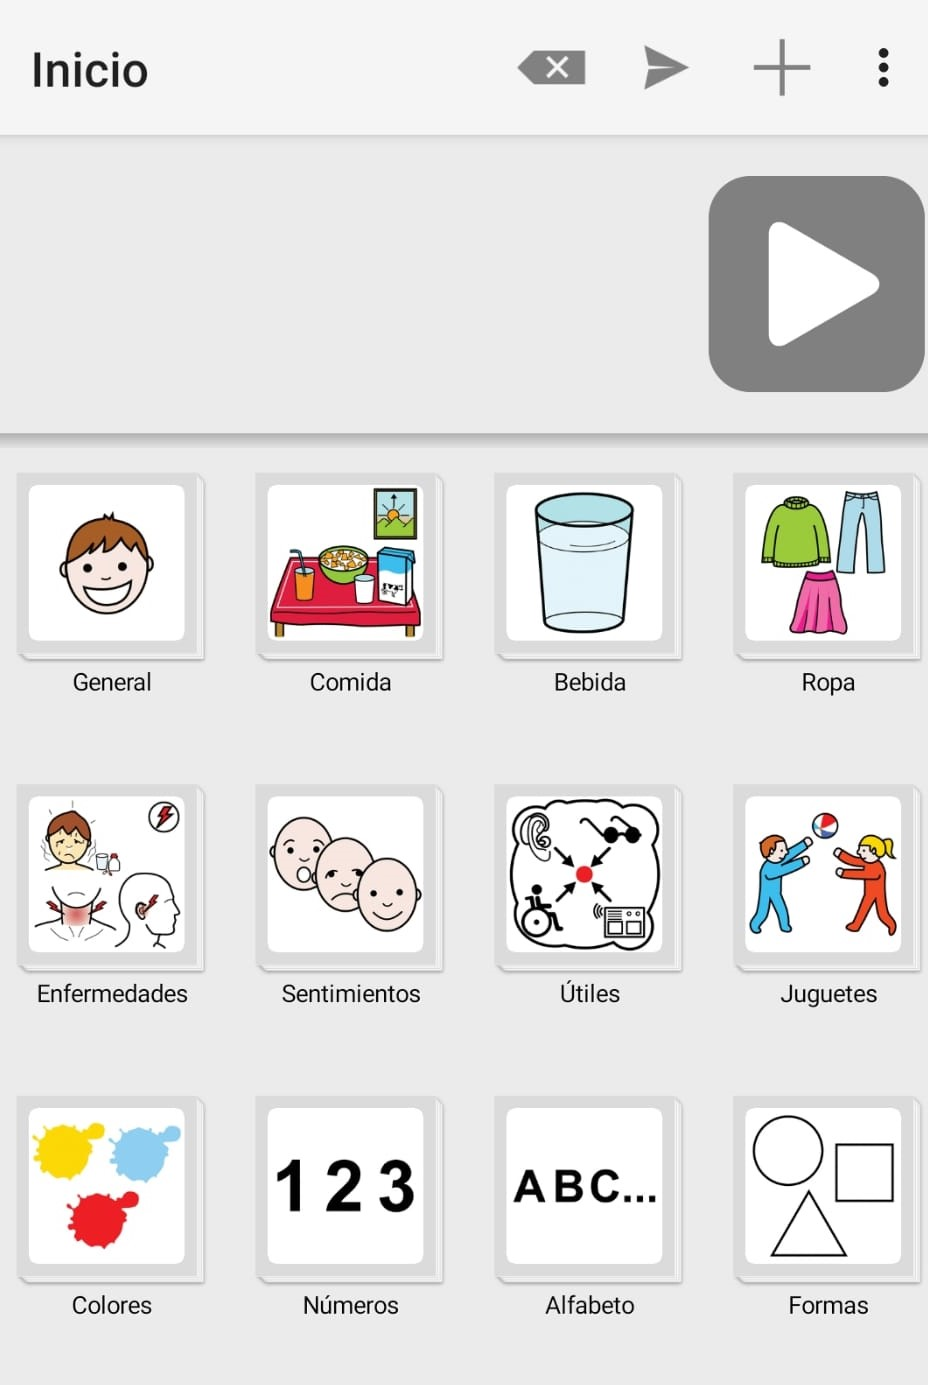
\includegraphics[width=0.7\linewidth]{Imagenes/Bitmap/LetMeTalk}
	\caption{Menú de la aplicación en Android de LetMe Talk.}
	\label{fig:letmetalk}
\end{figure}

\newpage

\section*{Análisis de los resultados}


Puestas todas las herramientas en comparación recopiladas en la Tabla \ref{tab:comparativa}, podemos extraer algunos resultados. Actualmente la mayoría de estas herramientas están disponibles y con una base de datos de pictogramas actualizada. Los más completos o que ofrecen más opciones, están disponibles para ordenadores aunque en dispositivos móviles hay mayor oferta  de aplicaciones, generalmente ofrecen pocas opciones. Además de las aplicaciones de dispositivos, las más actualizadas son las que se pueden acceder en formato web.

Aunque a pesar de todo, el factor determinante es el precio. Las aplicaciones que no son gratuitas suelen tener un precio desorbitado o que muchas familias o docentes no pueden permitirse, por ello que una aplicación sea gratuita es determinante. Respecto a los idiomas, destacan el español y el inglés como idiomas predominantes entre las aplicaciones. 

Como conclusión, creemos que la herramienta que desarrollemos debería cumplir las siguientes características. Debe ser gratuita, disponible desde navegador web, con edición de pictogramas, una base de datos de éstos actualizada y que esté disponible como mínimo en español e inglés. 

\begin{table}[]
	\centering
	\resizebox{14cm}{!} {
		\begin{tabular}{|l|l|l|l|l|l|l|}
			\hline
			
			\textbf{Programas} & \textbf{Disponible} & \textbf{Actualizado} & \textbf{Dispositivos} & \textbf{{\begin{tabular}[c]{@{}l@{}}\\ Permite editar \\ pictogramas \\ \\\end{tabular}}}  & \textbf{Precio} & \textbf{Idiomas} \\  \hline
			
			\textbf{Pictoselector} &Sí  &Sí  &PC y MAC  &Sí &Gratuito &{\begin{tabular}[c]{@{}l@{}}\\ES, EN, DU, FR, \\ PT, IT\\ \\\end{tabular}} \\ \hline
			\textbf{Editor ARASAAC} &Sí  &Sí  &{\begin{tabular}[c]{@{}l@{}}\\PC, MAC, Android, \\ iOS y Web \end{tabular}}  &Sí &Gratuito &{\begin{tabular}[c]{@{}l@{}}\\ES, EN, DU, FR, \\ PT, BZ, IT, RO, \\ PL, CN, AR, RU, \\ BG, CRO, NLD\\ \\\end{tabular}} \\ \hline
			\textbf{Piktoplus} &No  &No  &Android  &No &139€ &{\begin{tabular}[c]{@{}l@{}} \\ES \\ \\ \end{tabular}}\\ \hline
			\textbf{BoardMaker} &Sí  &Sí  &PC y MAC  &No &300€ &{\begin{tabular}[c]{@{}l@{}} \\ES, EN, PT \\ \\\end{tabular}}\\ \hline
			\textbf{Pictar} &Sí  &{\begin{tabular}[c]{@{}l@{}}\\La web no, \\los pictogramas sí\end{tabular}}  &Web  &No &Gratuito &{\begin{tabular}[c]{@{}l@{}} \\ES \\ \\ \end{tabular}}\\ \hline
			\textbf{Pictableros} &Sí  &{\begin{tabular}[c]{@{}l@{}}\\La web no, \\los pictogramas sí\end{tabular}}   &Web  &Sí &Gratuito &{\begin{tabular}[c]{@{}l@{}} \\ES \\ \\ \end{tabular}}\\ \hline
			\textbf{SymboTalk} &Sí  &No  &Web, Android e iOS  &No &Gratuito &{\begin{tabular}[c]{@{}l@{}} \\ES, EN, HEBR \\ \\ \end{tabular}}\\ \hline
			\textbf{LetMeTalk} &Sí  &No  &Android e iOS  &No &Gratuito &{\begin{tabular}[c]{@{}l@{}} \\ES, AR, DE, EN, \\ IT, FR, PL, PT, \\ RU, RO, SW, CN \\ \\\end{tabular}} \\ \hline
			
		\end{tabular}
	}
\caption{\label{tab:comparativa}Tabla comparativa entre los distintos editores de tableros basados en pictogramas}
\end{table}


%\include{Capitulos/Capitulo3}
%\include{Capitulos/Capitulo4}
%\include{Capitulos/Capitulo5}
\chapter{Conclusiones y Trabajo Futuro}
\label{cap:conclusiones}

\section{Conclusiones}
\label{cap7:sec:conclusiones}

El principal objetivo que se propuso de cara a la realización de este trabajo de fin de grado fue el poder realizar una aplicación web que facilitara la creación de materiales pictográficos, enfocado a la creación de tableros. Para ello nos informamos sobre los distintos tipos de sistemas pictográficos y qué personas solían utilizarlos. Tras una larga búsqueda vimos que el sistema pictográfico que mayor material proporcionaba era ARASAAC por lo que se decidió utilizar sus pictogramas para el desarrollo de la aplicación. Además la aplicación se desarrolló para cubrir ciertas carencias que otras aplicaciones de creación de tableros no tenían. Estas carencias solían ser funcionalidades como añadir imágenes propias al tablero, poder traducir una frase a pictogramas, añadir iconos o tener la posibilidad de tener los elementos del tablero fácilmente alineados. 

Tras desarrollar la aplicación se realizó una evaluación con usuarios para obtener datos referentes a la usabilidad y utilidad. Esta evaluación resultó de gran valor, ya que se pudo afirmar que la usabilidad es alta. Además se pudo contrastar qué funcionalidades se tenían que mejorar, además de conocer las opiniones de los usuarios, sobre los ya existentes.


Otro objetivo propuesto fue poder demostrar todos los conocimientos adquiridos durante la carrera y ampliarlos. Las asignaturas más influyentes para la realización del trabajo fin de grado fueron:

\begin{itemize}
	\item \textbf{Aplicaciones Web}: en esta asignatura se adquirieron conocimientos sobre HTML, Javascript y maquetación. Lo aprendido en JavaScript resultó de gran ayuda de cara al desarrollo de la aplicación en React. 
	
	\item\textbf{ Desarrollo de Sistemas Interactivos}: esta asignatura nos permitió conocer las diferentes formas de evaluación sobre una aplicación y ver la importancia de estas para detectar errores y ser solucionados.
	
	\item \textbf{Interfaces de usuario}: muy ligado al Desarrollo de Sistema Interactivos, esta asignatura nos permitió conocer reglas de diseño a seguir para crear interfaces intuitivas en la aplicación.
	
\end{itemize}


\section{Trabajo futuro}
\label{cap7:sec:trabajofuturo}
Una vez terminado el desarrollo de la aplicación y la evaluación de la misma, se recogieron las mejoras y nuevas funcionalidades que no pudieron ser implementadas y que sería interesante añadir en un futuro: 

\begin{itemize}
	\item Mejorar la funcionalidad de traducción de una frase a pictogramas mediante NIL-WS-API.
	\item Permitir al usuario poder guardar el estado de la aplicación por medio de Google Drive para posteriormente volver a cargar el estado del tablero y cargar imágenes que se encuentren en su cuenta.
	
	\item Implementar componentes interactivos, como subtableros o cajón de pictos.
	
	\item Ofrecer la posibilidad de poder ocultar la cuadrícula que se dibuja el tablero de la aplicación.
	\item Ofrecer la posibilidad de cambiar el tamaño del tablero.
	
	\item Implementar otro tipo de tablero que permita una edición más semejante a la ofrecida en Power Point, donde los elementos sobre el tablero puedan ser alineados con mayor facilidad.  
	\item Mejorar la interfaz en el apartado de las listas de pictogramas y traducción de frase a pictogramas para que tengan una mejor usabilidad.
	
	\item Añadir nuevos iconos que complementen a los pictogramas, como emoticonos que representen una cara feliz o triste.
	
	\item Ofrecer la posibilidad de añadir un vídeo al tablero y poder reproducirlo desde el mismo. Esto ayudaría al usuario a asociar un pictograma con una acción, por ejemplo con el pictograma de saltar junto a un gif de una persona saltando.
	
	\item Incluir un botón en la aplicación para borrar todos los elementos que estén en el tablero.
	
	\item Añadir un buscador de imágenes dentro de la web. Esto ayudaría a buscar imágenes de manera rápida evitando que el usuario tenga que descargar y subir las fotos a la web. 
	
	\item Posibilidad de asignar cualquier color al borde y fondo de un pictograma. El uso de los colores puede ser distinto dependiendo del usuario, por lo que se debe ofrecer la posibilidad de elegirlo libremente. 
	
\end{itemize}










%%%%%%%%%%%%%%%%%%%%%%%%%%%%%%%%%%%%%%%%%%%%%%%%%%%%%%%%%%%%%%%%%%%%%%%%%%%
% Si el TFM se escribe en inglés, comentar las siguientes líneas 
% porque no es necesario incluir nuevamente las Conclusiones en inglés
\setcounter{chapter}{\thechapter-1} 
\begin{otherlanguage}{english}
\chapter{Conclusions and Future Work}
\label{cap:conclusions}

\section{Conclusions}


The main objective that was proposed for the realization of this final degree project was to create a web application that would facilitate the creation of pictographic materials, focused on the creation of communication boards. To do this, we learned about the different types of pictographic systems and which people used to use them. After a long research, we saw that the pictographic system that had the biggest amount of pictograms was ARASAAC, so we decided to use their pictograms for the development of the application. In addition, the application was developed to cover certain gaps that other board creation applications did not have. These deficiencies used to be functionalities such as adding your own images to the board, being able to translate a sentence into pictograms, adding icons or the possibility to align easily and precisely the board elements.

After developing the application, an evaluation was carried out with users to obtain data regarding usability and usefulness. This evaluation was of great value, since it was possible to confirm that the usability was high. In addition, it was possible to contrast which functionalities had to be improved, in addition to knowing the opinions of the user about the existing ones.

Another proposed objective was to be able to demonstrate all the knowledge acquired during the degree and to expand it. The most influential subjects for the completion of the final degree project were:



\begin{itemize}
	\item Web applications: in this subject we acquired knowledge about HTML, JavaScript and layout. What we learned in JavaScript was of great help for the development of the application in React. 
	\item Development of interactive systems: this subject allowed us to learn about the different forms of evaluation on an application and to see the importance of these in order to detect errors and be solved.
	\item User Interfaces: closely linked to Interactive System Development, this subject allowed us to learn the design rules to follow to create intuitive interfaces in the application.
\end{itemize}



\section{Future work}

Once the development of the application and its evaluation were completed, we grouped the improvements and new functionalities that could not be implemented and that would be interesting to add in the future: 

\begin{itemize}
	\item Improve the functionality of translating a sentence to pictograms using NIL-WS-API.
	\item Allow the user to be able to save the state of the application through Google Drive to later reload the state of the board and upload images that are in their account.
	\item Implement interactive components, such as sub-boards or draggable pictograms that can be moved by the user to play a game.
	\item Offer the possibility to hide the grid that is drawn on the application's board.
	\item Offer the possibility to change the size of the board.
	\item Implement another type of board that allows an edition more similar to that offered in Power Point, where the elements on the board can be aligned more easily.  
	
	\item Improve the interface in the section of the pictogram lists and translation of sentence to pictograms for better usability.
	
	\item Add new icons to complement the pictograms, such as emoticons representing a happy or sad face.
	
	\item Offer the possibility of adding a video to the board and being able to play it from the board. This would help the user to associate a pictogram with an action, for example with the pictogram of jumping next to a gif of a person jumping.
	
	\item Include a button in the application to delete all the elements that are on the board.
	
	\item Add an image search engine within the website. This would help to search images quickly avoiding the user having to download and upload the photos to the web. 
	
	\item Possibility of assigning any color to the border and background of a pictogram. The use of colors can be different depending on the user, so the possibility of free choice should be offered. 
	
\end{itemize}









\end{otherlanguage}
%%%%%%%%%%%%%%%%%%%%%%%%%%%%%%%%%%%%%%%%%%%%%%%%%%%%%%%%%%%%%%%%%%%%%%%%%%%


% Apéndices
\appendix
\chapter{Título}
\label{Appendix:Key1}

Contenido del apéndice
\chapter{Título}
\label{Appendix:Key2}

%\include{Apendices/appendixC}
%\include{...}
%\include{...}
%\include{...}
\backmatter

%
% Bibliografía
%
% Si el TFM se escribe en inglés, editar TeXiS/TeXiS_bib para cambiar el
% estilo de las referencias
%---------------------------------------------------------------------
%
%                      configBibliografia.tex
%
%---------------------------------------------------------------------
%
% bibliografia.tex
% Copyright 2009 Marco Antonio Gomez-Martin, Pedro Pablo Gomez-Martin
%
% This file belongs to the TeXiS manual, a LaTeX template for writting
% Thesis and other documents. The complete last TeXiS package can
% be obtained from http://gaia.fdi.ucm.es/projects/texis/
%
% Although the TeXiS template itself is distributed under the 
% conditions of the LaTeX Project Public License
% (http://www.latex-project.org/lppl.txt), the manual content
% uses the CC-BY-SA license that stays that you are free:
%
%    - to share & to copy, distribute and transmit the work
%    - to remix and to adapt the work
%
% under the following conditions:
%
%    - Attribution: you must attribute the work in the manner
%      specified by the author or licensor (but not in any way that
%      suggests that they endorse you or your use of the work).
%    - Share Alike: if you alter, transform, or build upon this
%      work, you may distribute the resulting work only under the
%      same, similar or a compatible license.
%
% The complete license is available in
% http://creativecommons.org/licenses/by-sa/3.0/legalcode
%
%---------------------------------------------------------------------
%
% Fichero  que  configura  los  parámetros  de  la  generación  de  la
% bibliografía.  Existen dos  parámetros configurables:  los ficheros
% .bib que se utilizan y la frase célebre que aparece justo antes de la
% primera referencia.
%
%---------------------------------------------------------------------


%%%%%%%%%%%%%%%%%%%%%%%%%%%%%%%%%%%%%%%%%%%%%%%%%%%%%%%%%%%%%%%%%%%%%%
% Definición de los ficheros .bib utilizados:
% \setBibFiles{<lista ficheros sin extension, separados por comas>}
% Nota:
% Es IMPORTANTE que los ficheros estén en la misma línea que
% el comando \setBibFiles. Si se desea utilizar varias líneas,
% terminarlas con una apertura de comentario.
%%%%%%%%%%%%%%%%%%%%%%%%%%%%%%%%%%%%%%%%%%%%%%%%%%%%%%%%%%%%%%%%%%%%%%
\setBibFiles{%
nuestros,latex,otros%
}


%%%%%%%%%%%%%%%%%%%%%%%%%%%%%%%%%%%%%%%%%%%%%%%%%%%%%%%%%%%%%%%%%%%%%%
% Definición de la frase célebre para el capítulo de la
% bibliografía. Dentro normalmente se querrá hacer uso del entorno
% \begin{FraseCelebre}, que contendrá a su vez otros dos entornos,
% un \begin{Frase} y un \begin{Fuente}.
%
% Nota:
% Si no se quiere cita, se puede eliminar su definición (en la
% macro setCitaBibliografia{} ).
%%%%%%%%%%%%%%%%%%%%%%%%%%%%%%%%%%%%%%%%%%%%%%%%%%%%%%%%%%%%%%%%%%%%%%


%%
%% Creamos la bibliografia
%%
\makeBib

% Variable local para emacs, para  que encuentre el fichero maestro de
% compilación y funcionen mejor algunas teclas rápidas de AucTeX

%%%
%%% Local Variables:
%%% mode: latex
%%% TeX-master: "../Tesis.tex"
%%% End:

%
% Índice de palabras
%

% Sólo  la   generamos  si  está   declarada  \generaindice.  Consulta
% TeXiS.sty para más información.

% En realidad, el soporte para la generación de índices de palabras
% en TeXiS no está documentada en el manual, porque no ha sido usada
% "en producción". Por tanto, el fichero que genera el índice
% *no* se incluye aquí (está comentado). Consulta la documentación
% en TeXiS_pream.tex para más información.
\ifx\generaindice\undefined
\else
%%---------------------------------------------------------------------
%
%                        TeXiS_indice.tex
%
%---------------------------------------------------------------------
%
% TeXiS_indice.tex
% Copyright 2009 Marco Antonio Gomez-Martin, Pedro Pablo Gomez-Martin
%
% This file belongs to TeXiS, a LaTeX template for writting
% Thesis and other documents. The complete last TeXiS package can
% be obtained from http://gaia.fdi.ucm.es/projects/texis/
%
% This work may be distributed and/or modified under the
% conditions of the LaTeX Project Public License, either version 1.3
% of this license or (at your option) any later version.
% The latest version of this license is in
%   http://www.latex-project.org/lppl.txt
% and version 1.3 or later is part of all distributions of LaTeX
% version 2005/12/01 or later.
%
% This work has the LPPL maintenance status `maintained'.
% 
% The Current Maintainers of this work are Marco Antonio Gomez-Martin
% and Pedro Pablo Gomez-Martin
%
%---------------------------------------------------------------------
%
% Contiene  los  comandos  para  generar  el índice  de  palabras  del
% documento.
%
%---------------------------------------------------------------------
%
% NOTA IMPORTANTE: el  soporte en TeXiS para el  índice de palabras es
% embrionario, y  de hecho  ni siquiera se  describe en el  manual. Se
% proporciona  una infraestructura  básica (sin  terminar)  para ello,
% pero  no ha  sido usada  "en producción".  De hecho,  a pesar  de la
% existencia de  este fichero, *no* se incluye  en Tesis.tex. Consulta
% la documentación en TeXiS_pream.tex para más información.
%
%---------------------------------------------------------------------


% Si se  va a generar  la tabla de  contenidos (el índice  habitual) y
% también vamos a  generar el índice de palabras  (ambas decisiones se
% toman en  función de  la definición  o no de  un par  de constantes,
% puedes consultar modo.tex para más información), entonces metemos en
% la tabla de contenidos una  entrada para marcar la página donde está
% el índice de palabras.

\ifx\generatoc\undefined
\else
   \addcontentsline{toc}{chapter}{\indexname}
\fi


% Generamos el índice
\printindex

% Variable local para emacs, para  que encuentre el fichero maestro de
% compilación y funcionen mejor algunas teclas rápidas de AucTeX

%%%
%%% Local Variables:
%%% mode: latex
%%% TeX-master: "./tesis.tex"
%%% End:

\fi

%
% Lista de acrónimos
%

% Sólo  lo  generamos  si  está declarada  \generaacronimos.  Consulta
% TeXiS.sty para más información.


\ifx\generaacronimos\undefined
\else
%---------------------------------------------------------------------
%
%                        TeXiS_acron.tex
%
%---------------------------------------------------------------------
%
% TeXiS_acron.tex
% Copyright 2009 Marco Antonio Gomez-Martin, Pedro Pablo Gomez-Martin
%
% This file belongs to TeXiS, a LaTeX template for writting
% Thesis and other documents. The complete last TeXiS package can
% be obtained from http://gaia.fdi.ucm.es/projects/texis/
%
% This work may be distributed and/or modified under the
% conditions of the LaTeX Project Public License, either version 1.3
% of this license or (at your option) any later version.
% The latest version of this license is in
%   http://www.latex-project.org/lppl.txt
% and version 1.3 or later is part of all distributions of LaTeX
% version 2005/12/01 or later.
%
% This work has the LPPL maintenance status `maintained'.
% 
% The Current Maintainers of this work are Marco Antonio Gomez-Martin
% and Pedro Pablo Gomez-Martin
%
%---------------------------------------------------------------------
%
% Contiene  los  comandos  para  generar  el listado de acrónimos
% documento.
%
%---------------------------------------------------------------------
%
% NOTA IMPORTANTE:  para que la  generación de acrónimos  funcione, al
% menos  debe  existir  un  acrónimo   en  el  documento.  Si  no,  la
% compilación  del   fichero  LaTeX  falla  con   un  error  "extraño"
% (indicando  que  quizá  falte  un \item).   Consulta  el  comentario
% referente al paquete glosstex en TeXiS_pream.tex.
%
%---------------------------------------------------------------------


% Redefinimos a español  el título de la lista  de acrónimos (Babel no
% lo hace por nosotros esta vez)

\def\listacronymname{Lista de acrónimos}

% Para el glosario:
% \def\glosarryname{Glosario}

% Si se  va a generar  la tabla de  contenidos (el índice  habitual) y
% también vamos a  generar la lista de acrónimos  (ambas decisiones se
% toman en  función de  la definición  o no de  un par  de constantes,
% puedes consultar config.tex  para más información), entonces metemos
% en la  tabla de contenidos una  entrada para marcar  la página donde
% está el índice de palabras.

\ifx\generatoc\undefined
\else
   \addcontentsline{toc}{chapter}{\listacronymname}
\fi


% Generamos la lista de acrónimos (en realidad el índice asociado a la
% lista "acr" de GlossTeX)

\printglosstex(acr)

% Variable local para emacs, para  que encuentre el fichero maestro de
% compilación y funcionen mejor algunas teclas rápidas de AucTeX

%%%
%%% Local Variables:
%%% mode: latex
%%% TeX-master: "../Tesis.tex"
%%% End:

\fi

%
% Final
%
%---------------------------------------------------------------------
%
%                      fin.tex
%
%---------------------------------------------------------------------
%
% fin.tex
% Copyright 2009 Marco Antonio Gomez-Martin, Pedro Pablo Gomez-Martin
%
% This file belongs to the TeXiS manual, a LaTeX template for writting
% Thesis and other documents. The complete last TeXiS package can
% be obtained from http://gaia.fdi.ucm.es/projects/texis/
%
% Although the TeXiS template itself is distributed under the 
% conditions of the LaTeX Project Public License
% (http://www.latex-project.org/lppl.txt), the manual content
% uses the CC-BY-SA license that stays that you are free:
%
%    - to share & to copy, distribute and transmit the work
%    - to remix and to adapt the work
%
% under the following conditions:
%
%    - Attribution: you must attribute the work in the manner
%      specified by the author or licensor (but not in any way that
%      suggests that they endorse you or your use of the work).
%    - Share Alike: if you alter, transform, or build upon this
%      work, you may distribute the resulting work only under the
%      same, similar or a compatible license.
%
% The complete license is available in
% http://creativecommons.org/licenses/by-sa/3.0/legalcode
%
%---------------------------------------------------------------------
%
% Contiene la última página
%
%---------------------------------------------------------------------


% Ponemos el marcador en el PDF
\ifpdf
   \pdfbookmark{Fin}{fin}
\fi

\thispagestyle{empty}\mbox{}

\vspace*{4cm}

\small

\hfill \emph{--¿Qué te parece desto, Sancho? -- Dijo Don Quijote --}

\hfill \emph{Bien podrán los encantadores quitarme la ventura,}

\hfill \emph{pero el esfuerzo y el ánimo, será imposible.}

\hfill 

\hfill \emph{Segunda parte del Ingenioso Caballero} 

\hfill \emph{Don Quijote de la Mancha}

\hfill \emph{Miguel de Cervantes}

\vfill%space*{4cm}

\hfill \emph{--Buena está -- dijo Sancho --; fírmela vuestra merced.}

\hfill \emph{--No es menester firmarla -- dijo Don Quijote--,}

\hfill \emph{sino solamente poner mi rúbrica.}

\hfill 

\hfill \emph{Primera parte del Ingenioso Caballero} 

\hfill \emph{Don Quijote de la Mancha}

\hfill \emph{Miguel de Cervantes}


\newpage
\thispagestyle{empty}\mbox{}

\newpage

% Variable local para emacs, para  que encuentre el fichero maestro de
% compilación y funcionen mejor algunas teclas rápidas de AucTeX

%%%
%%% Local Variables:
%%% mode: latex
%%% TeX-master: "../Tesis.tex"
%%% End:

%\end{otherlanguage}
\end{document}
